%\thispagestyle{empty}
\footnotesize
% Setup and stylize appendices to integrate with TOC
\addtocontents{toc}{\protect\renewcommand\protect\cftchappresnum{\appendixname~}}
\renewcommand{\thechapter}{\Roman{chapter}}

% Stylize section header
\renewcommand{\thesection}{\Alph{section}}

% Appendix I: Oligonucleotide and probe sequences
%\addcontentsline{toc}{chapter}{Oligonucleotide and probe sequences}
\chapter{The Macroeconomic Consequences of Unemployment Scarring}


\pagebreak 


\section{Appendix I}

\subsection{Simulating The 1980s, 1990-91, and 2000s Recessions}

In this section, I explore whether scarring can explain the recoveries of all other recessions since the 1980s. For each recession, I assume the steady state of the model is the quarter in which the given recession begins and recalibrate $\zeta^{X}$ to match the proportion of the increase in the unemployment rate due to permanent layoffs, temporary layoffs, and quits/others that is estimated in \cite{Gertler2022} and from the decomposition of unemployment flows constructed by \cite{Fujita2017}. In addition, I fix the real wage by setting $\phi_{w} =1$.  I then repeat the estimation procedure for simulating the Great Recession without estimating monetary policy shocks for parsimony. In addition, for each recession, the data are detrended from the end of the previous recession up until beginning of the next recession.\footnote{ Pushing back the beginning of the detrending interval to be 20 years before the beginning of the recession makes little difference to the results. }

\subsubsection{The 80s Recession}

The model suggests that scarring played a limited role in explaining the recovery of consumption and output from the recessions in the 80s. Figure \ref{80s_recession} plots the responses of the unemployment rate, hourly labor compensation, consumption and GDP against the data. The responses represent deviations from 1980Q1, the beginning of the first recession of the 80s. From the figure, the model with scarring has difficulty accounting for the response of consumption but can account for the long run behavior of output. The path of hourly labor compensation provides a good fit to the data until 1985. The model has difficulty accounting for the path of hourly labor compensation after 1985 because it cannot capture the compositional changes of hourly labor compensation due to the absence of working hours as well as not having the job separation rate depend on human capital.  

\begin{figure}[H] % "[t!]" placement specifier just for this example
\centering
\begin{minipage}{0.51\textwidth}
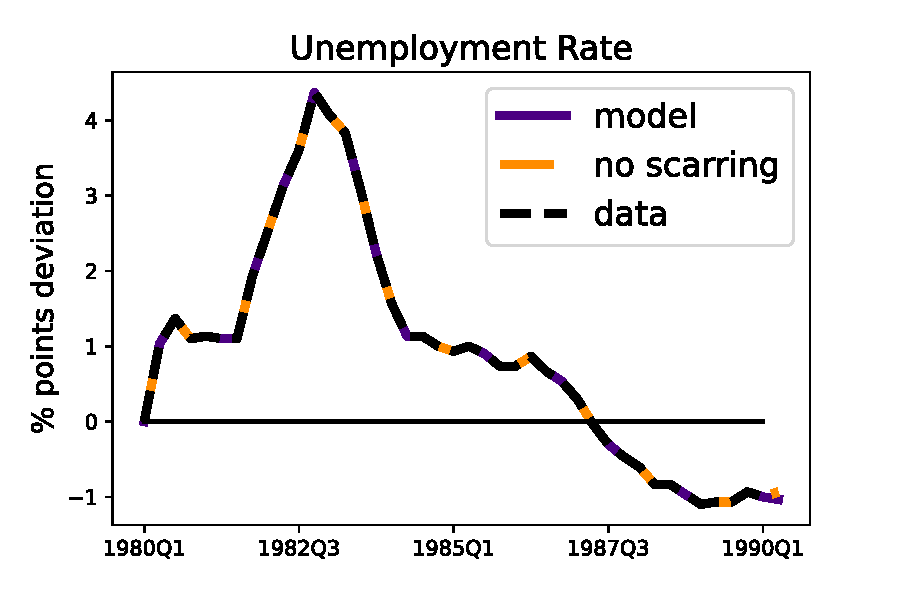
\includegraphics[scale=.57]{text/Chapter1/Figures/80s/Urate_80s}
\end{minipage}\hspace*{\fill}
\begin{minipage}{0.51\textwidth}
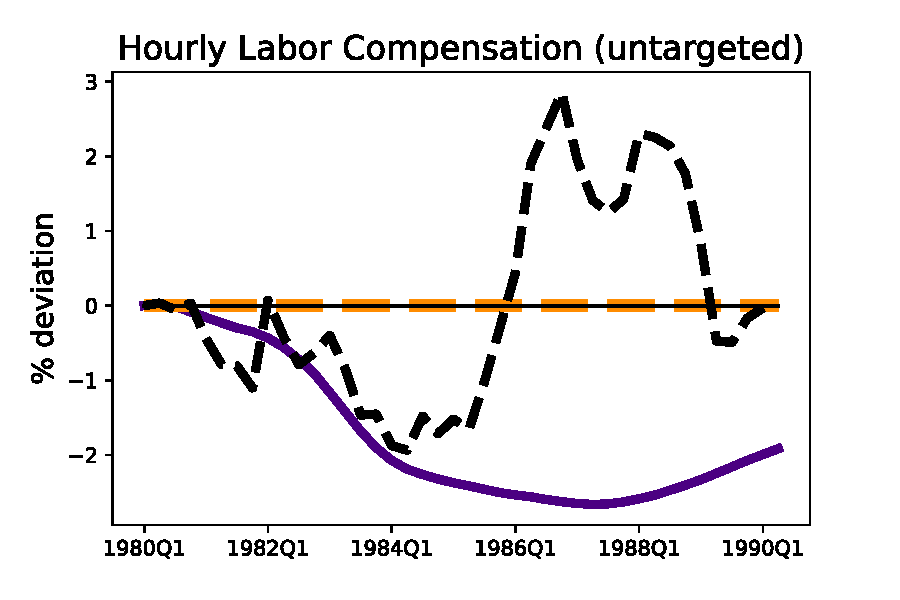
\includegraphics[scale=.57]{text/Chapter1/Figures/80s/hourly_comp_80s}
\end{minipage}

\medskip
\begin{minipage}{0.51\textwidth}
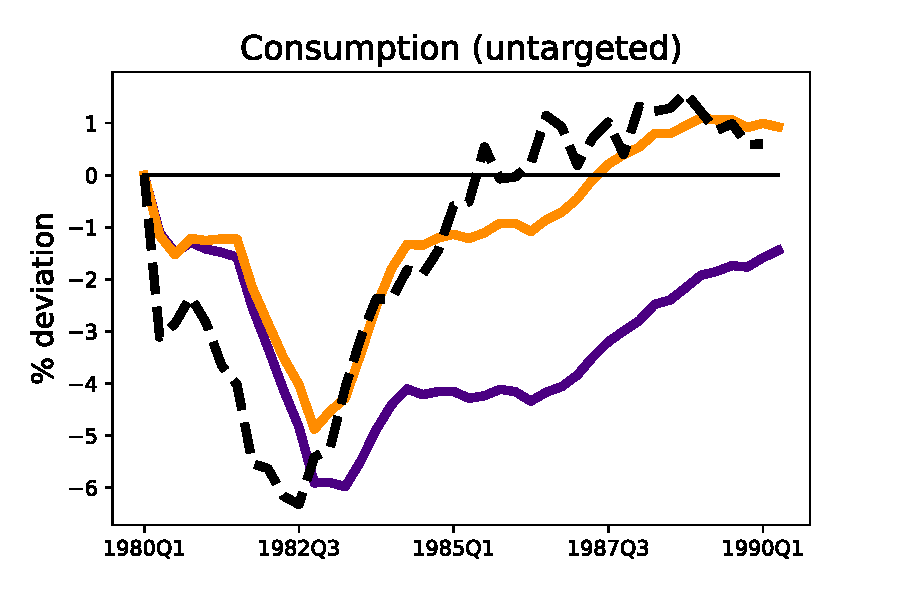
\includegraphics[scale=.57]{text/Chapter1/Figures/80s/PCE_IPR_80s}
\end{minipage}\hspace*{\fill}
\begin{minipage}{0.51\textwidth}
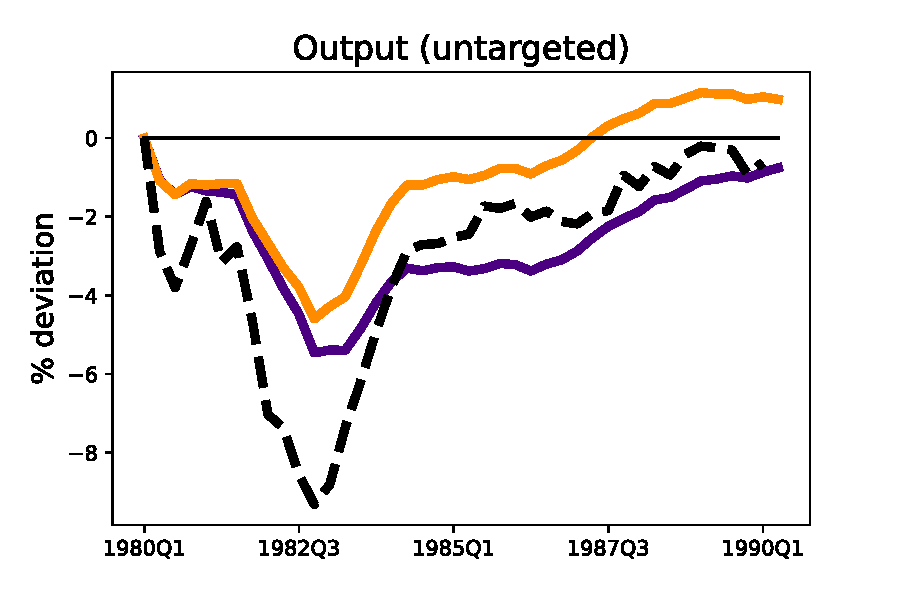
\includegraphics[scale=.57]{text/Chapter1/Figures/80s/GDP_IPR_80s}
\end{minipage}
\caption{Model vs data: 1980s}
\label{80s_recession}
\end{figure}





\subsubsection{The 1990-1991 Recession}

According to the model, scarring plays an important role in explaining the recovery from the 1990s recession. Figure \ref{90s_recession} plots the responses for the 1990-1991 recession against the data. The responses represent deviations from 1990Q3. With scarring, the model matches the responses of consumption and GDP well as well as matching the overall trend in hourly labor compensation. The response of hourly labor compensation likely rises in the beginning due lower wage workers being fired first. As mentioned previously, the model does not capture this fact.




\begin{figure}[H] % "[t!]" placement specifier just for this example
\centering
\begin{minipage}{0.51\textwidth}
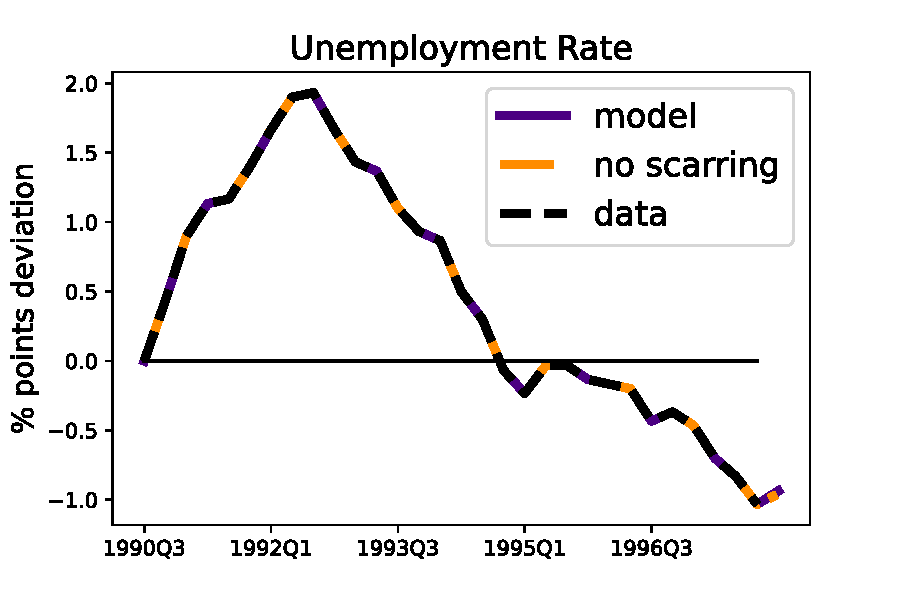
\includegraphics[scale=.57]{text/Chapter1/Figures/90s/Urate_90s}
 \label{fig:a}
\end{minipage}\hspace*{\fill}
\begin{minipage}{0.51\textwidth}
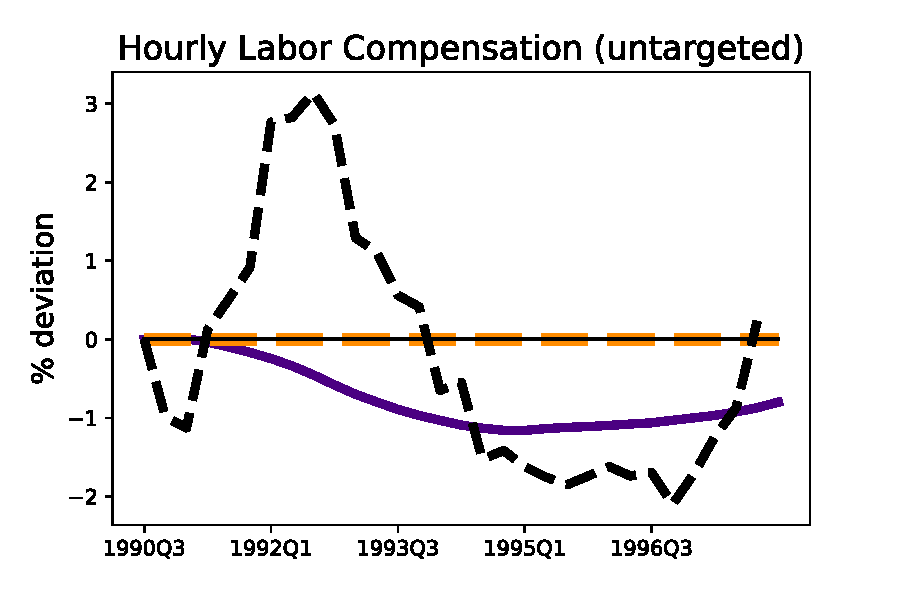
\includegraphics[scale=.57]{text/Chapter1/Figures/90s/hourly_comp_83Q1}
 \label{fig:b}
\end{minipage}

\medskip
\begin{minipage}{0.51\textwidth}
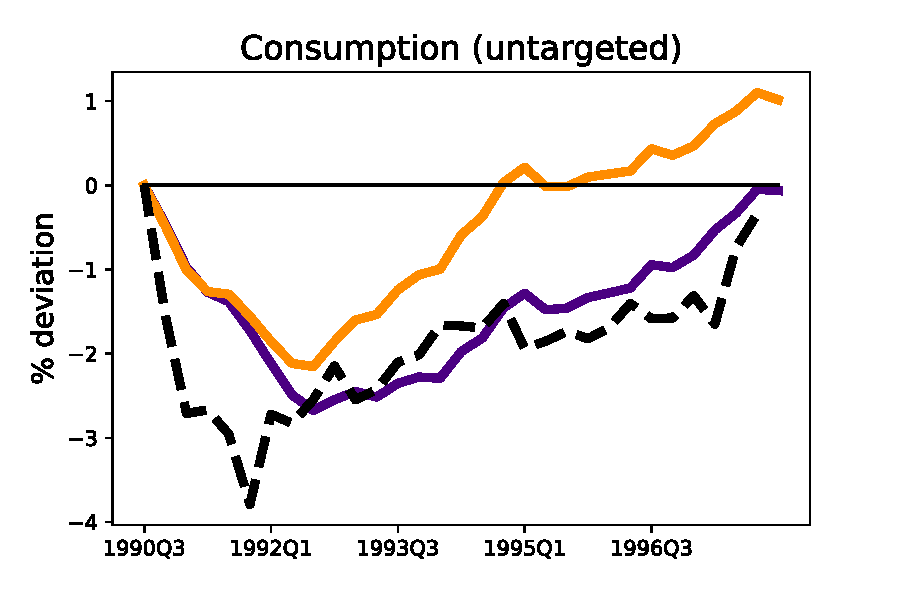
\includegraphics[scale=.57]{text/Chapter1/Figures/90s/PCE_IPR_90s_83Q1}
\label{fig:c}
\end{minipage}\hspace*{\fill}
\begin{minipage}{0.51\textwidth}
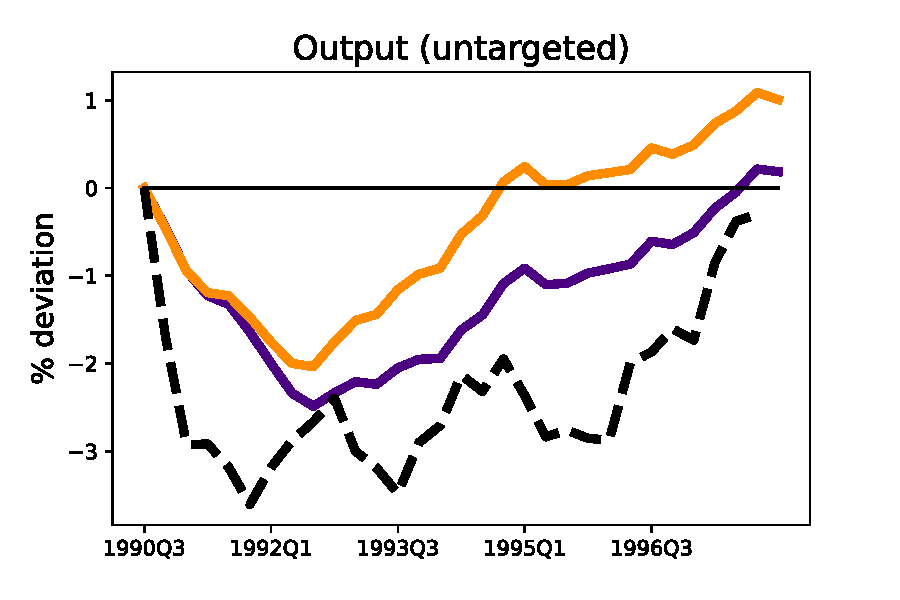
\includegraphics[scale=.57]{text/Chapter1/Figures/90s/GDP_IPR_90s_83Q1}
 \label{fig:d}
\end{minipage}
\caption{Model vs data: 1990-1991 recession}
\label{90s_recession}
\end{figure}

\subsubsection{The 2001 Recession}

Similar to the 1990-1991 recession, scarring can help explain the recovery from the 2001 recession. Figure \ref{00s_recessions} plots the responses for the 2001 recession against the data. The responses represent deviations from 2001Q2. With scarring, the model can help explain the long run behavior of consumption and GDP. The model also captures the trend in hourly labor compensation seen in the data. 



\begin{figure}[H] % "[t!]" placement specifier just for this example
\centering
\begin{minipage}{0.51\textwidth}
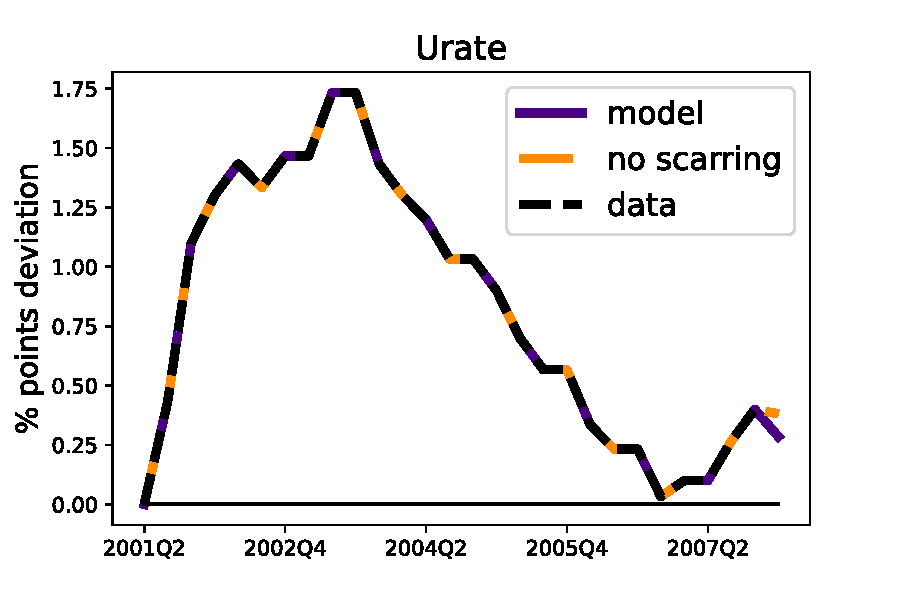
\includegraphics[scale=.57]{text/Chapter1/Figures/2000s/Urate_00s}
\end{minipage}\hspace*{\fill}
\begin{minipage}{0.51\textwidth}
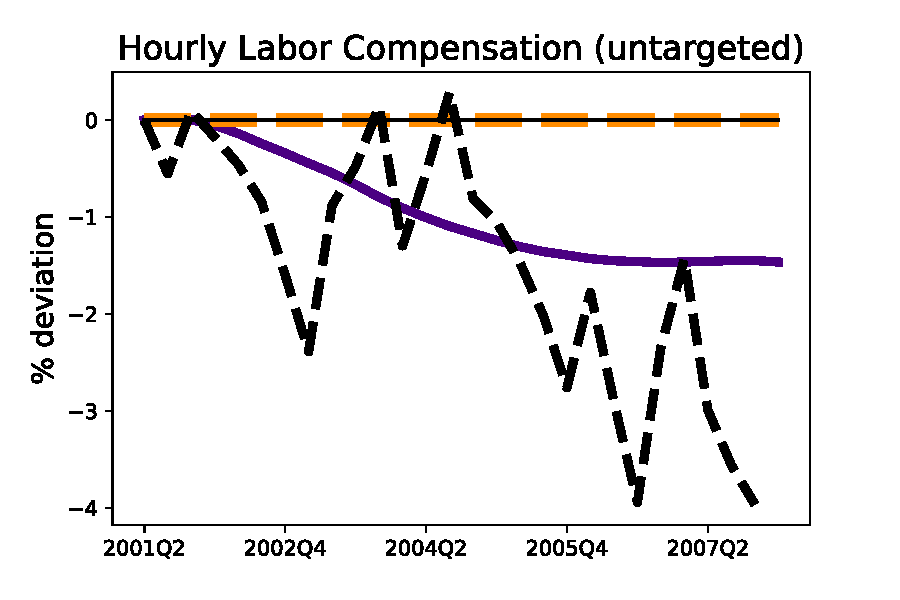
\includegraphics[scale=.57]{text/Chapter1/Figures/2000s/hourly_comp_00s}
\end{minipage}

\medskip
\begin{minipage}{0.51\textwidth}
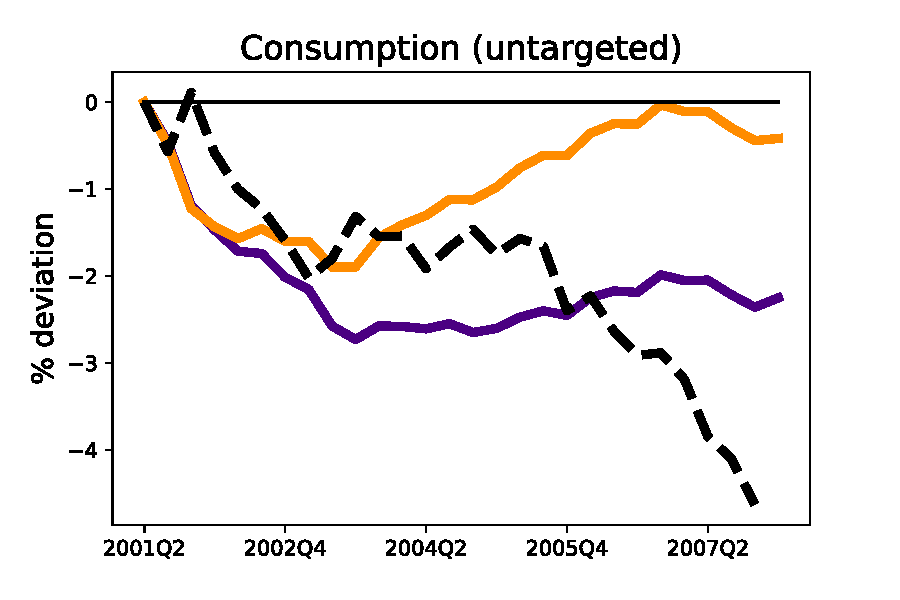
\includegraphics[scale=.57]{text/Chapter1/Figures/2000s/PCE_00s}
\end{minipage}\hspace*{\fill}
\begin{minipage}{0.51\textwidth}
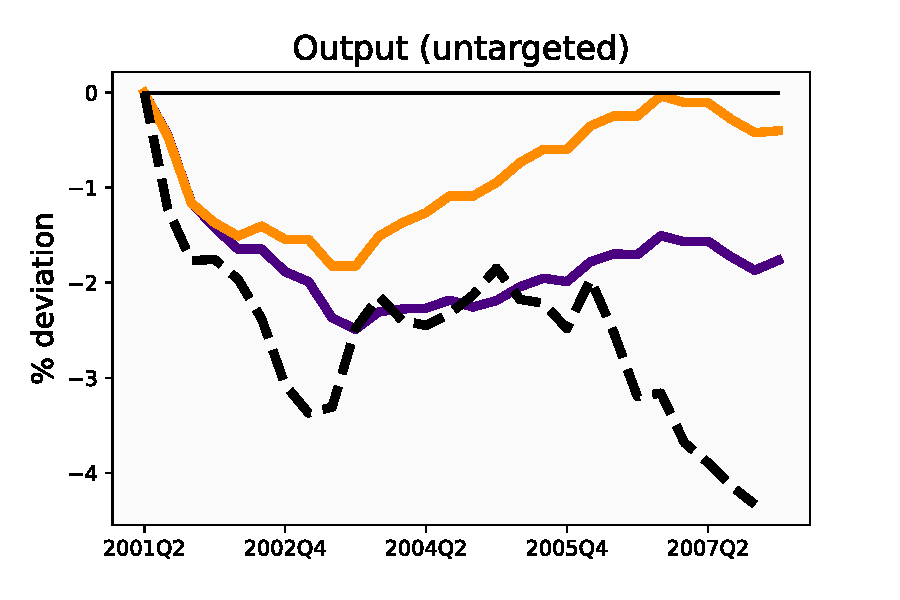
\includegraphics[scale=.57]{text/Chapter1/Figures/2000s/GDP_00s}
\end{minipage}
\caption{Model vs data: 2000s}
\label{00s_recessions}
\end{figure}






\subsection{Unemployment Risk as an Amplifier of Business Cycles}
\label{appendix:Urisk}

Precautionary saving in response to heightened unemployment risk is larger in the presence of scarring. This greater intensity in precautionary behavior leads unemployment risk to be a larger amplifier of business cycles. Figure \ref{Urisk_base} (baseline calibration) and figure \ref{Urisk_base_fixed_wage} (fixed real wage) plot the response of consumption to the negative demand shock from section 6.1 with and without perceived unemployment risk under the baseline model and the model with no scarring. The plots demonstrate that unemployment risk is a larger amplifier of business cycles, especially under a fixed real wage.  Increased precautionary saving in response to heightened unemployment risk dampens consumption, reduces labor demand, and therefore further raises the unemployment rate. This sequence of events is self reinforcing as the increase in the unemployment rate further increases precautionary saving. When households perceive that unemployment can lead to scars, this channel is substantially larger,




\begin{figure}[H]
    \centering
   \begin{minipage}{0.47\textwidth}
        \centering
        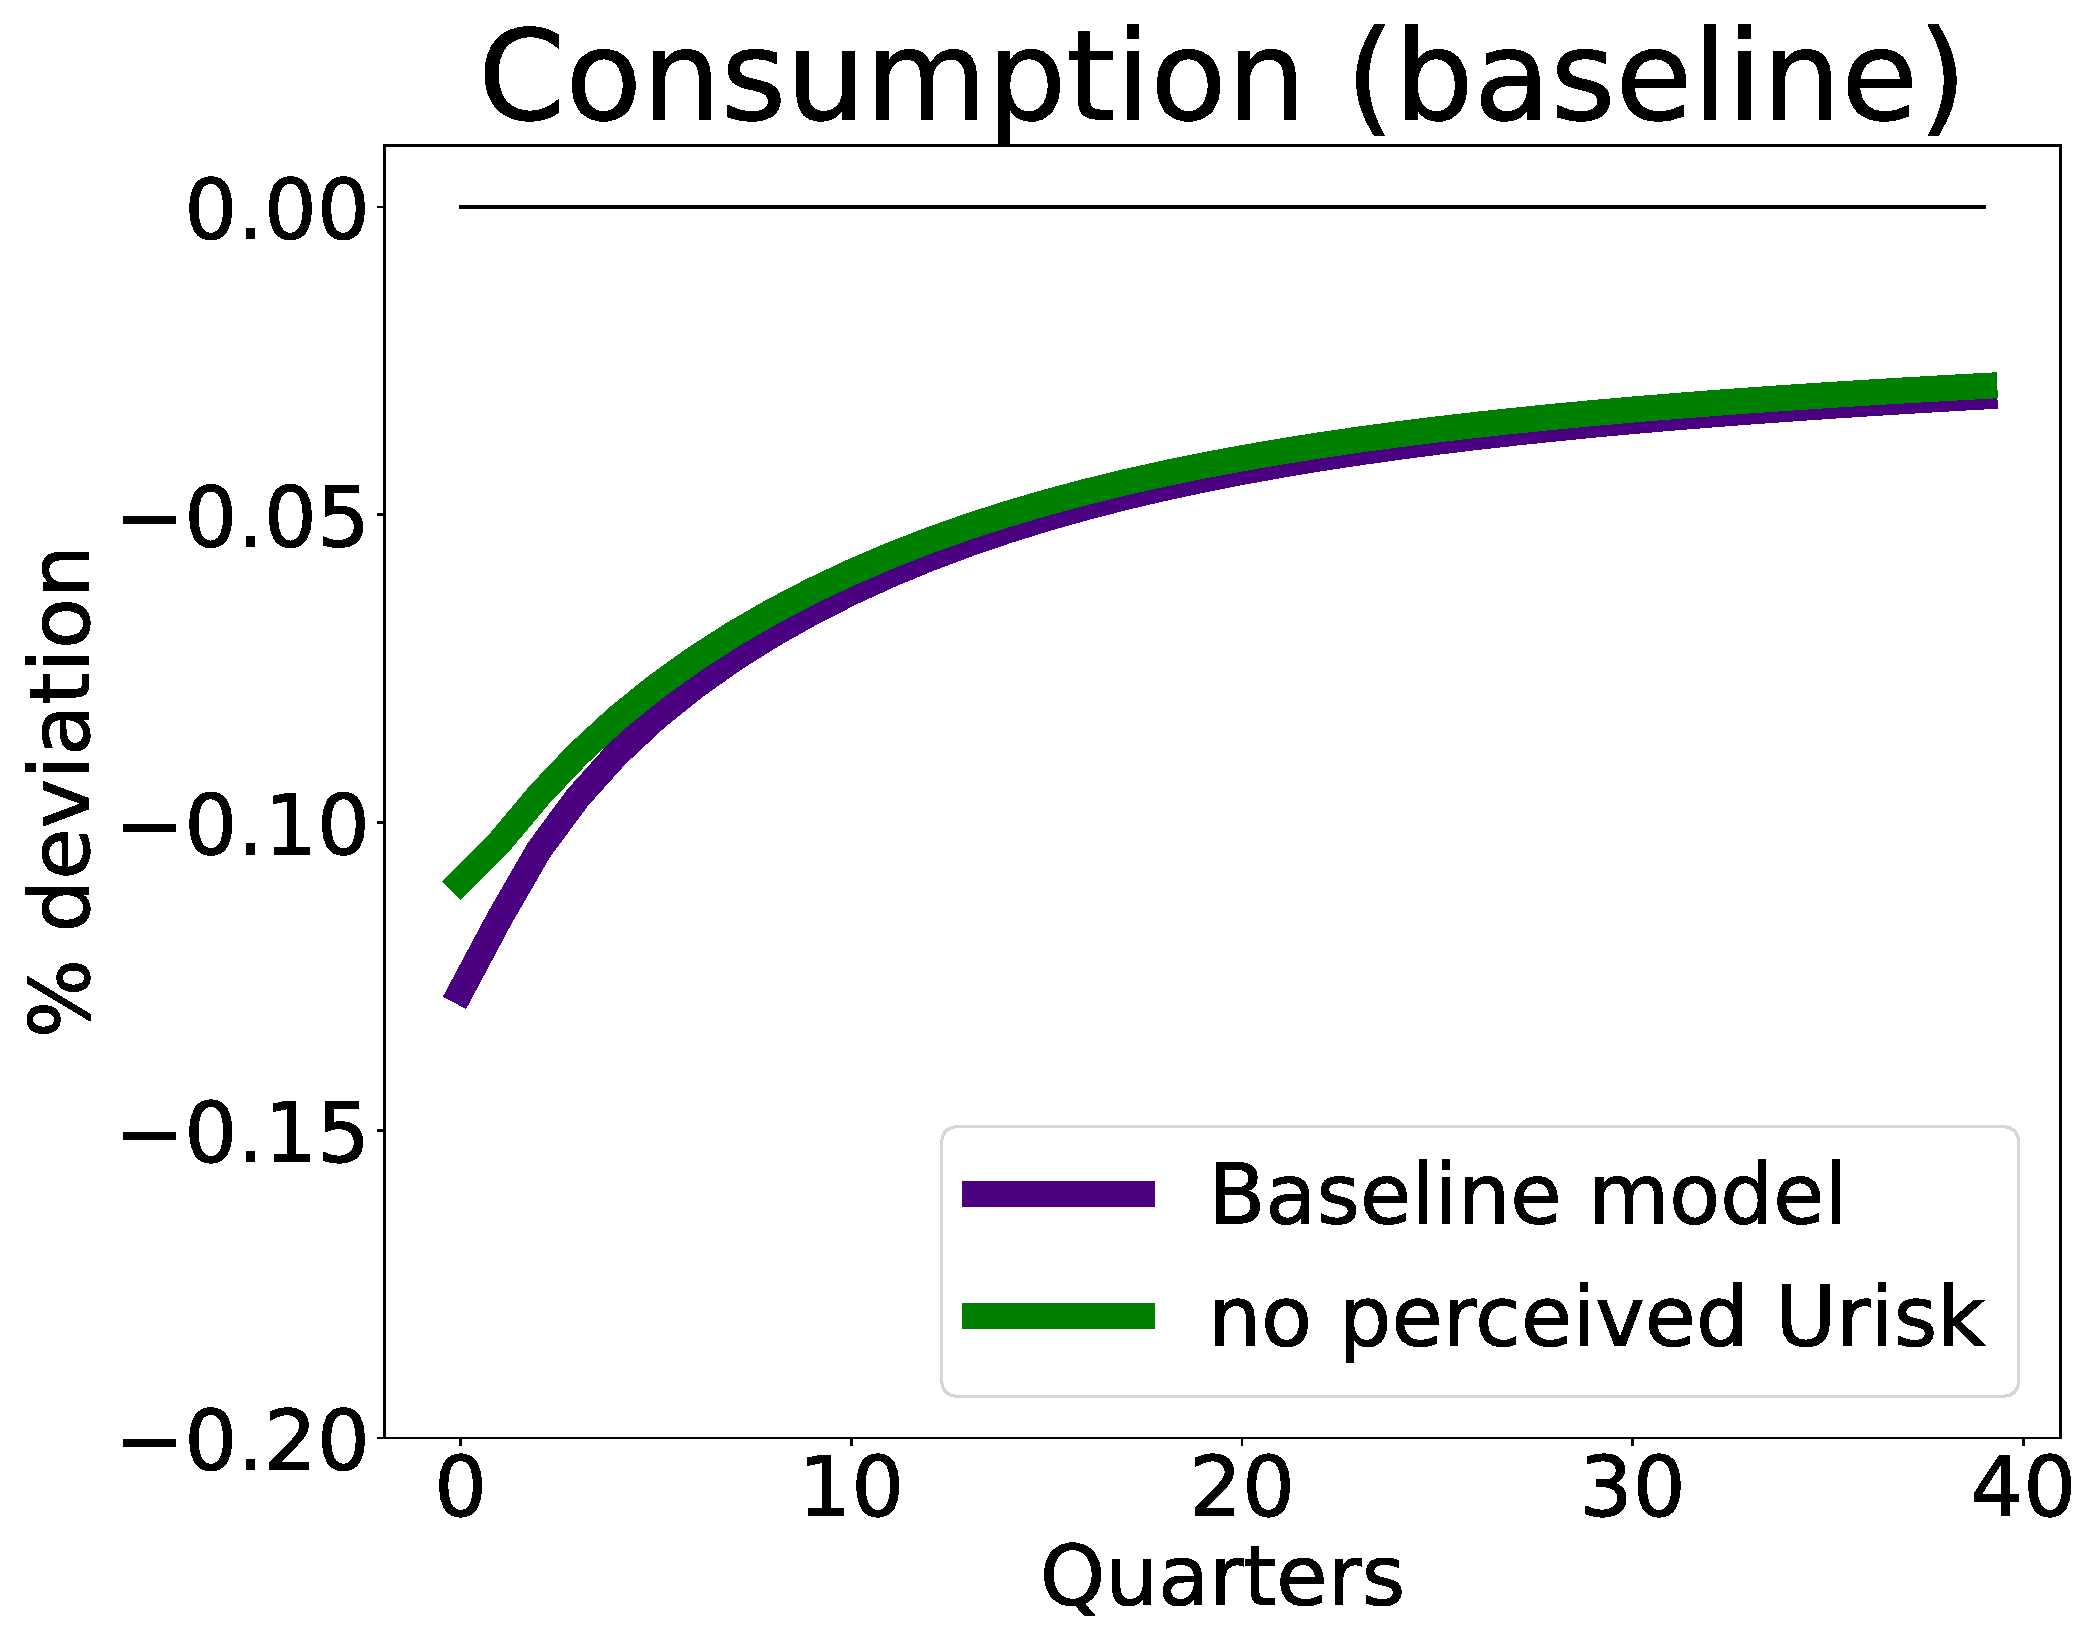
\includegraphics[scale=.2]{text/Chapter1/Figures/Urisk/C_IPR_urisk_base_flex_wage} % first figure itself
    \end{minipage}\hfill
    \begin{minipage}{0.47\textwidth}
        \centering
        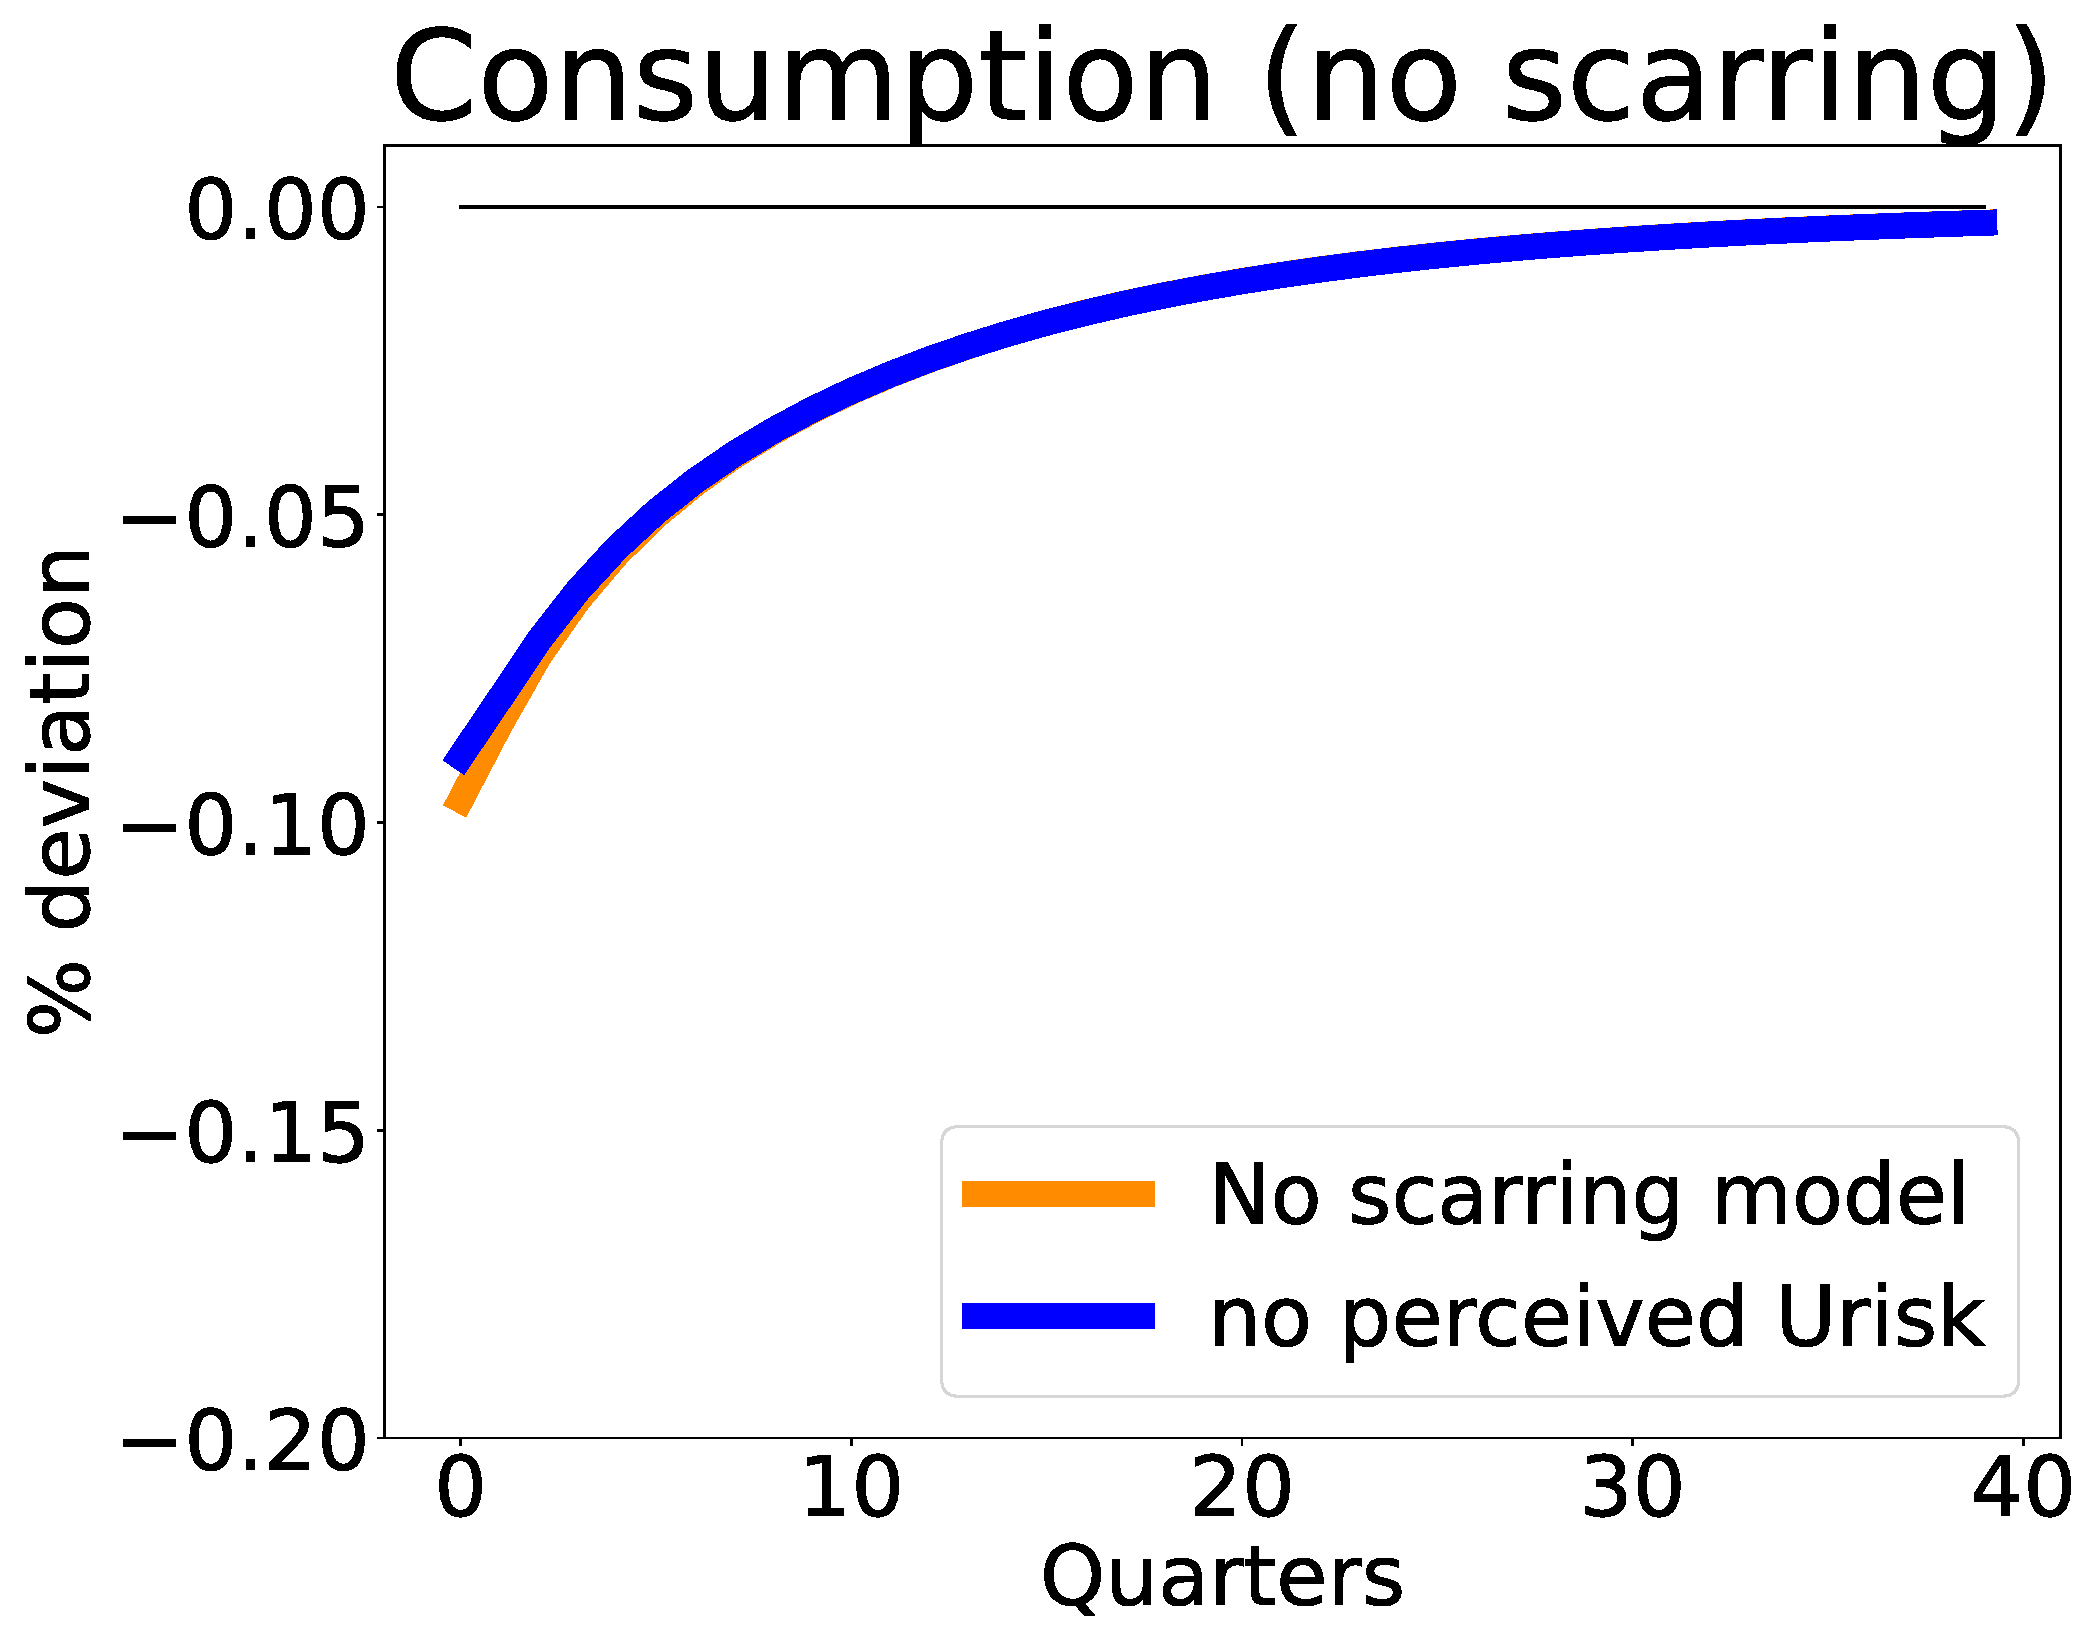
\includegraphics[scale=.2]{text/Chapter1/Figures/Urisk/C_IPR_urisk_base_no_scar_flex_wage} % second figure itself
    \end{minipage}
    \caption{Responses of Consumption to demand shock with and without perceived unemployment risk.}
    \label{Urisk_base}
\end{figure}




\begin{figure}[!ht]
    \centering
   \begin{minipage}{0.47\textwidth}
        \centering
        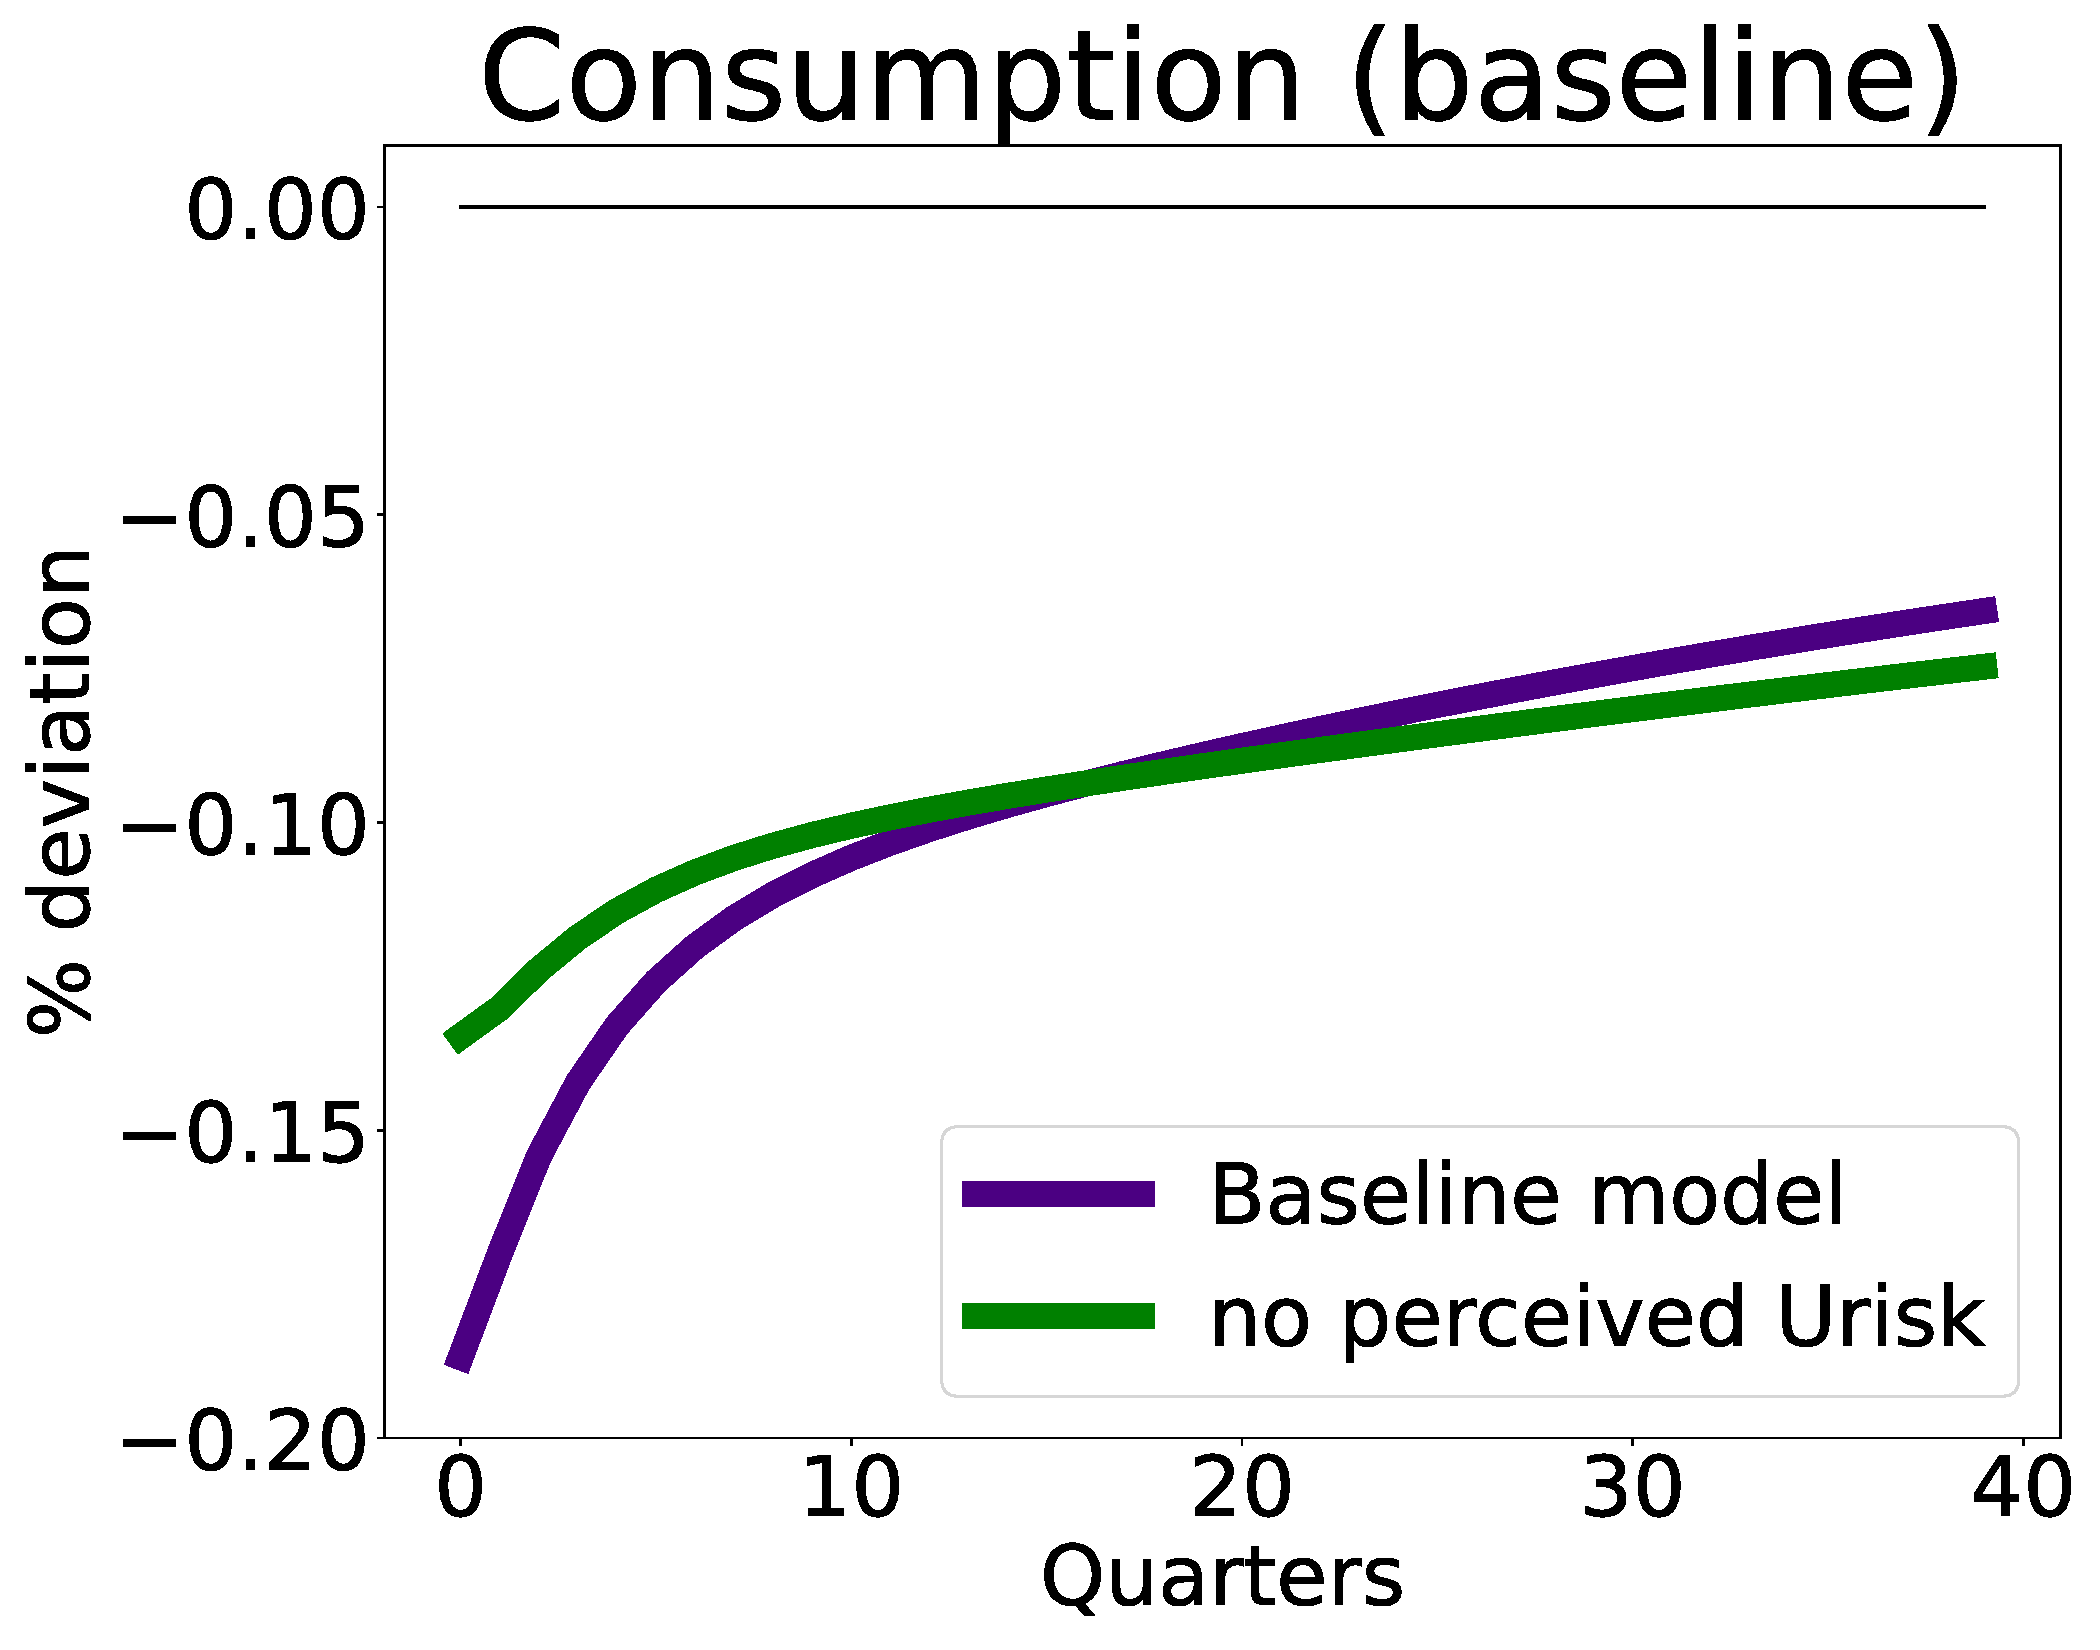
\includegraphics[scale=.2]{text/Chapter1/Figures/Urisk/C_IPR_urisk_base_fixed_wage} % first figure itself
    \end{minipage}\hfill
    \begin{minipage}{0.47\textwidth}
        \centering
        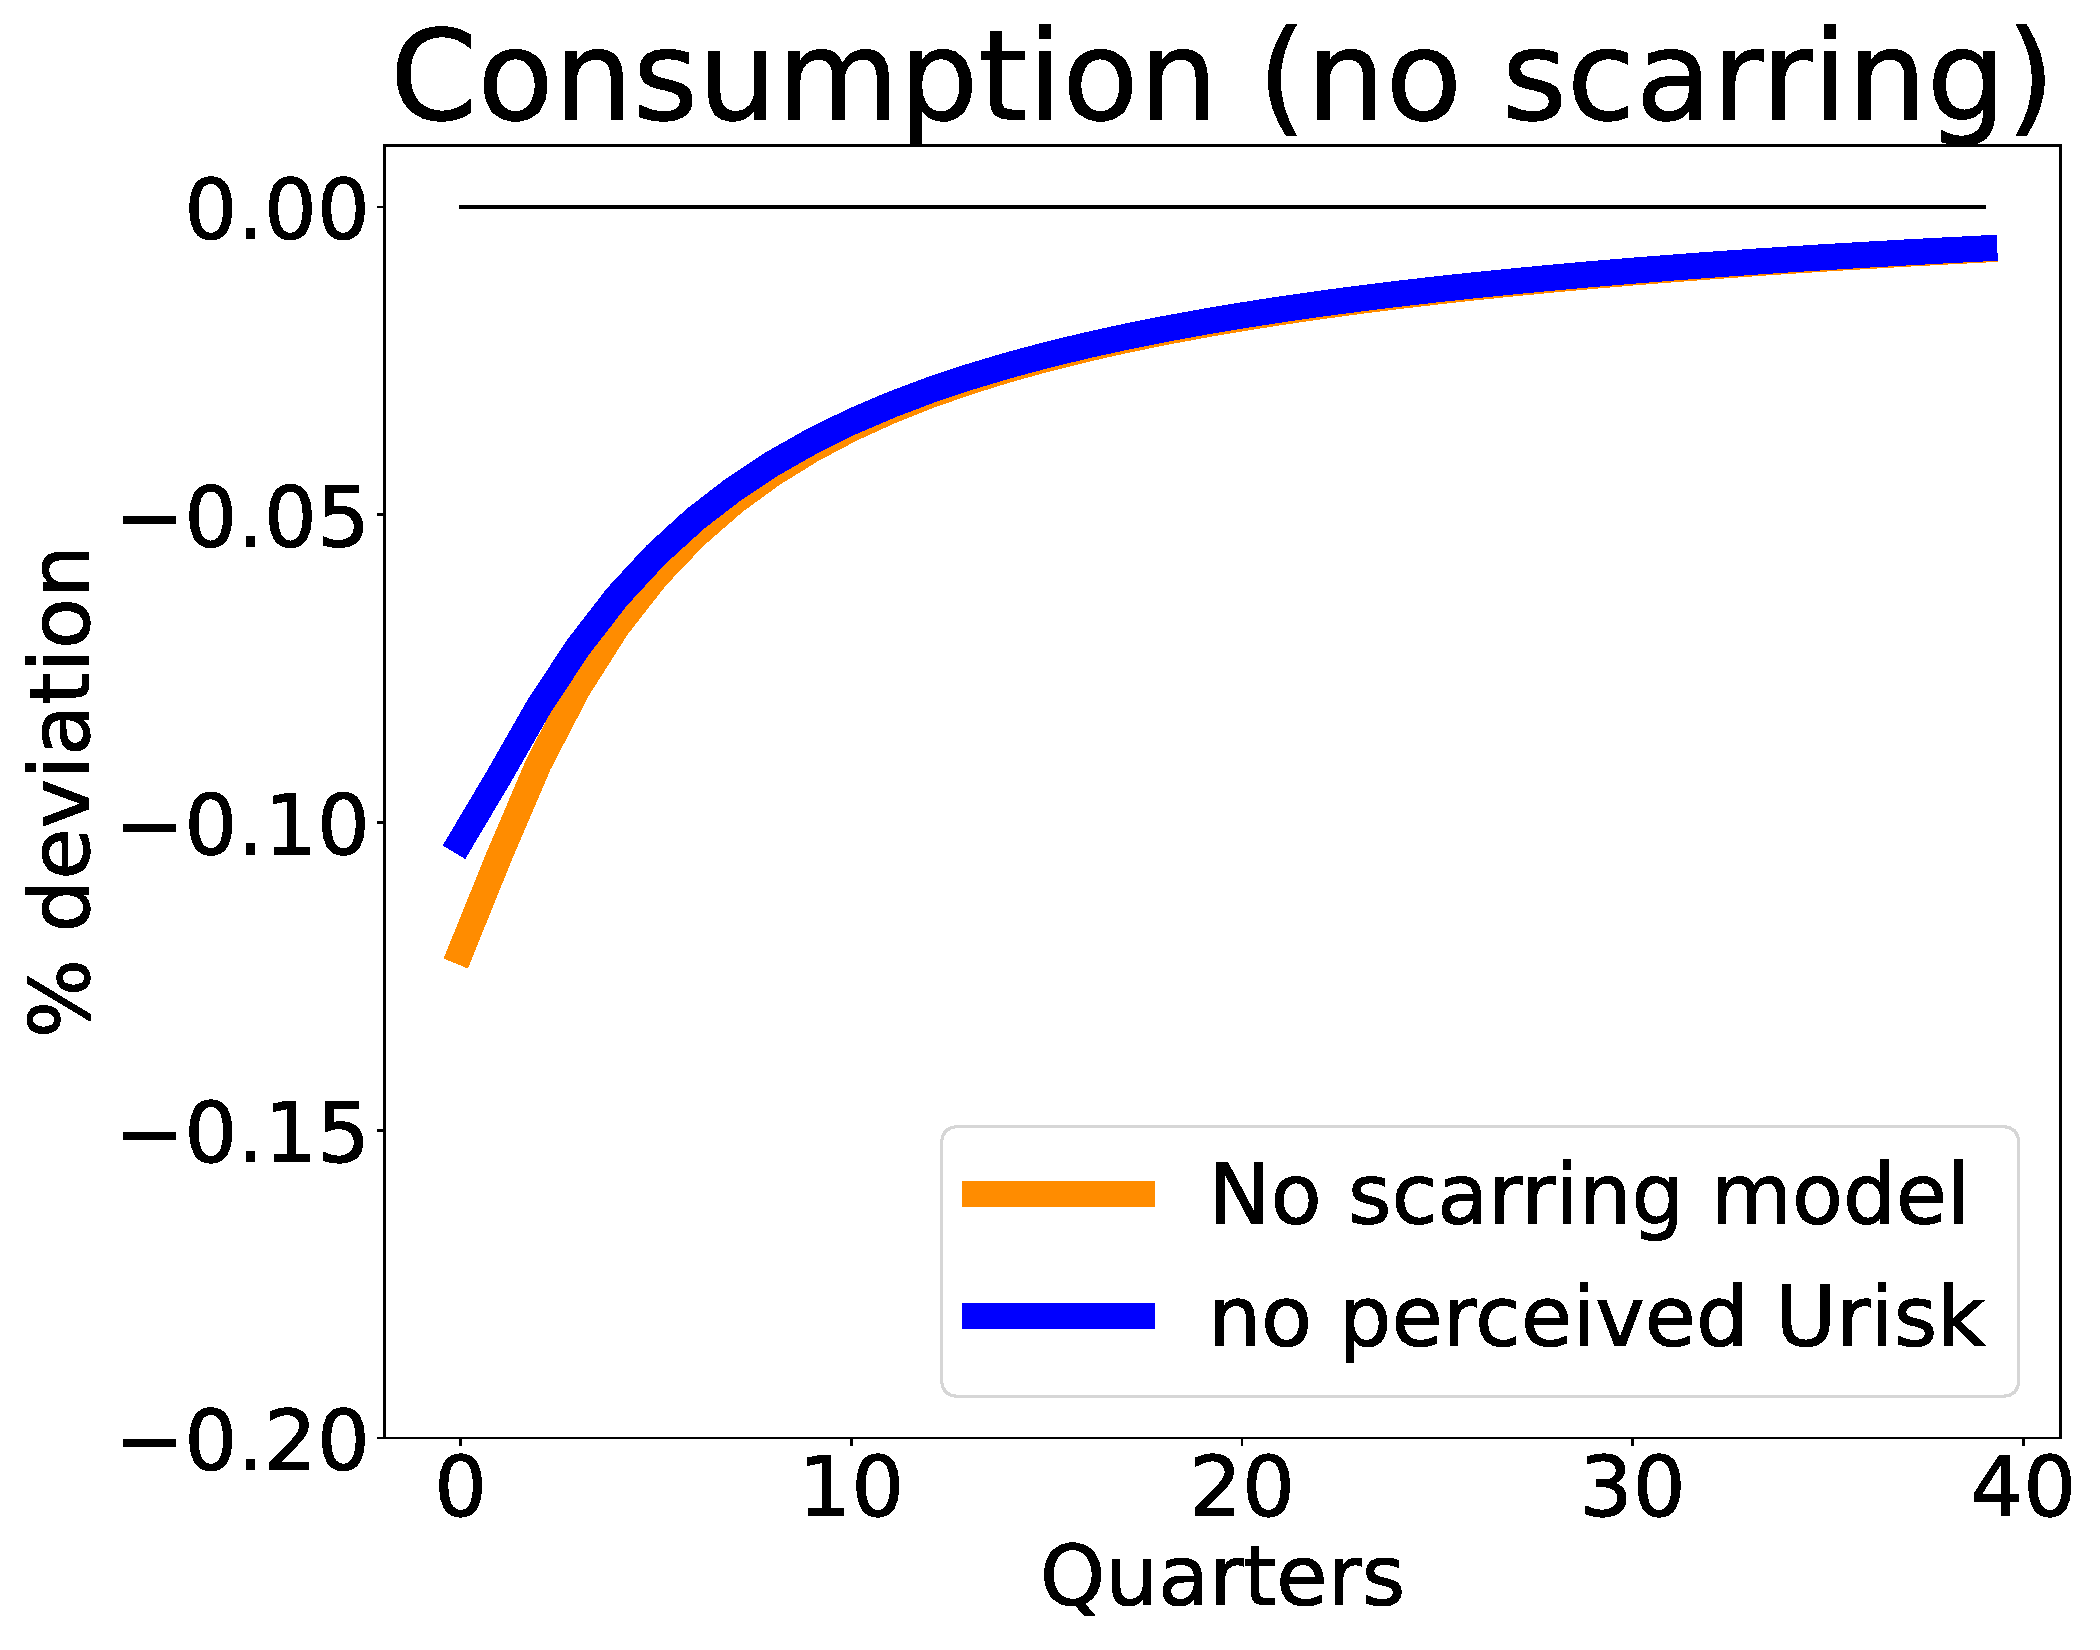
\includegraphics[scale=.2]{text/Chapter1/Figures/Urisk/C_IPR_urisk_base_no_scar_fixed_wage} % second figure itself
    \end{minipage}
    \caption{Responses of Consumption to demand shock under a fixed real wage with and without perceived unemployment risk.}
    \floatfoot{Note: The response of consumption in the baseline model is less persistent than its counterpart without scarring because the response of precautionary saving is front loaded in a model with perfect foresight. To be specific, in response to the negative demand shock, the decumulation of precautionary savings after $t=0$ is larger in the model with scarring because their buffer stocks were substantially large to begin with. This decumulation is large enough to to reduce the persistence of consumption.}

    \label{Urisk_base_fixed_wage}
\end{figure}






\subsection{Using other shocks to simulate the Great Recession}

This section demonstrates that the choice of shock chosen to match the unemployment rate during the Great Recession in figure \ref{Estimatedshks} does not matter. I consider a price markup shock and a shock to the variance of permanent income. For each type of shock, I estimate innovations to the respective variable to match the unemployment rate.  Figure \ref{other_shocks} plots the responses of consumption and output when either shock process is estimated to match the unemployment rate during the Great Recession.
\begin{figure}[!ht]
    \centering
   \begin{minipage}{0.47\textwidth}
        \centering
        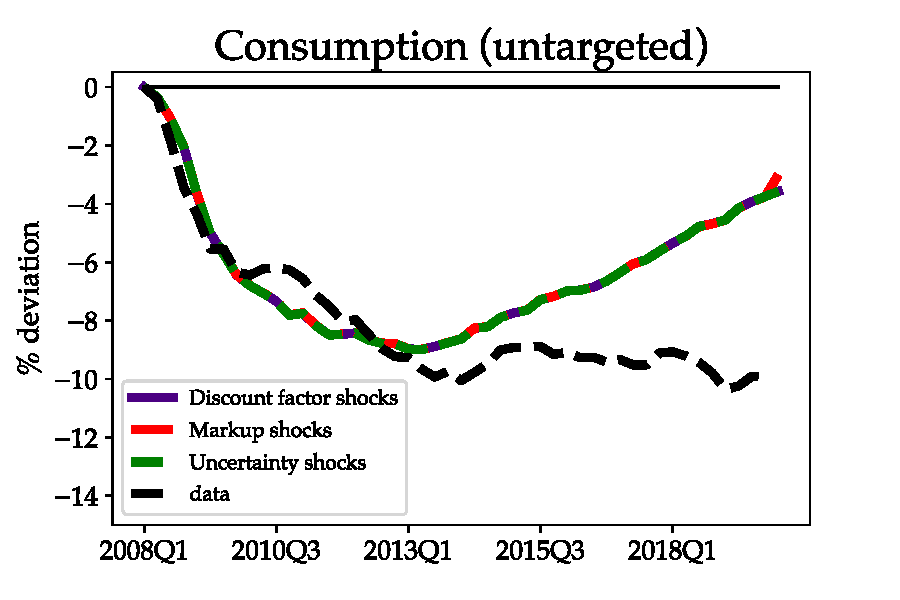
\includegraphics[scale=.6]{text/Chapter1/Figures/GR_sim/C_comparisons} % first figure itself
    \end{minipage}\hfill
    \caption{Simulation of Great Recession Using different shocks.}
    \label{other_shocks}
\end{figure}







\subsection{Monetary Policy and Unemployment Scarring}
\label{appendix:MP}

This section demonstrates that monetary policy exerts persistent effects on output, aggregate labor productivity, and income inequality when unemployment scarring is present. Figure \ref{IPR_ev} plots the impulse responses to a 25 basis point shock to the Taylor rule. The results reveal that monetary policy triggers enduring responses in output, mean human capital, and the Gini index for income. For this analysis, I modify the Taylor rule to include inertia: 


$$i_{t} = r^{*} + \phi_{ev} i_{t-1} + (1-\phi_{ev})(\phi_{\pi} \pi_{t} + \phi_{Y} (Y_{t} - Y_{ss})) + \epsilon^{m}_{t}$$

where the inertial parameter $\phi_{ev}$ is calibrated to 0.8. The persistent impulse responses to a monetary tightening align with the findings of \cite{Jorda2023}, who show that monetary contractions produce lasting declines in output without a prolonged increase in the unemployment rate. The key mechanism is that unemployment scarring results in a permanent decline in workers' human capital. Consequently, this scarring effect does not cause an extended rise in unemployment but instead transmits to output through a persistent reduction in aggregate labor productivity. As a result, unemployment scarring offers an alternative rationale for the empirical results in \cite{Jorda2023}.





\begin{figure}[htb]
    \centering % <-- added
\begin{minipage}{0.33\textwidth}
  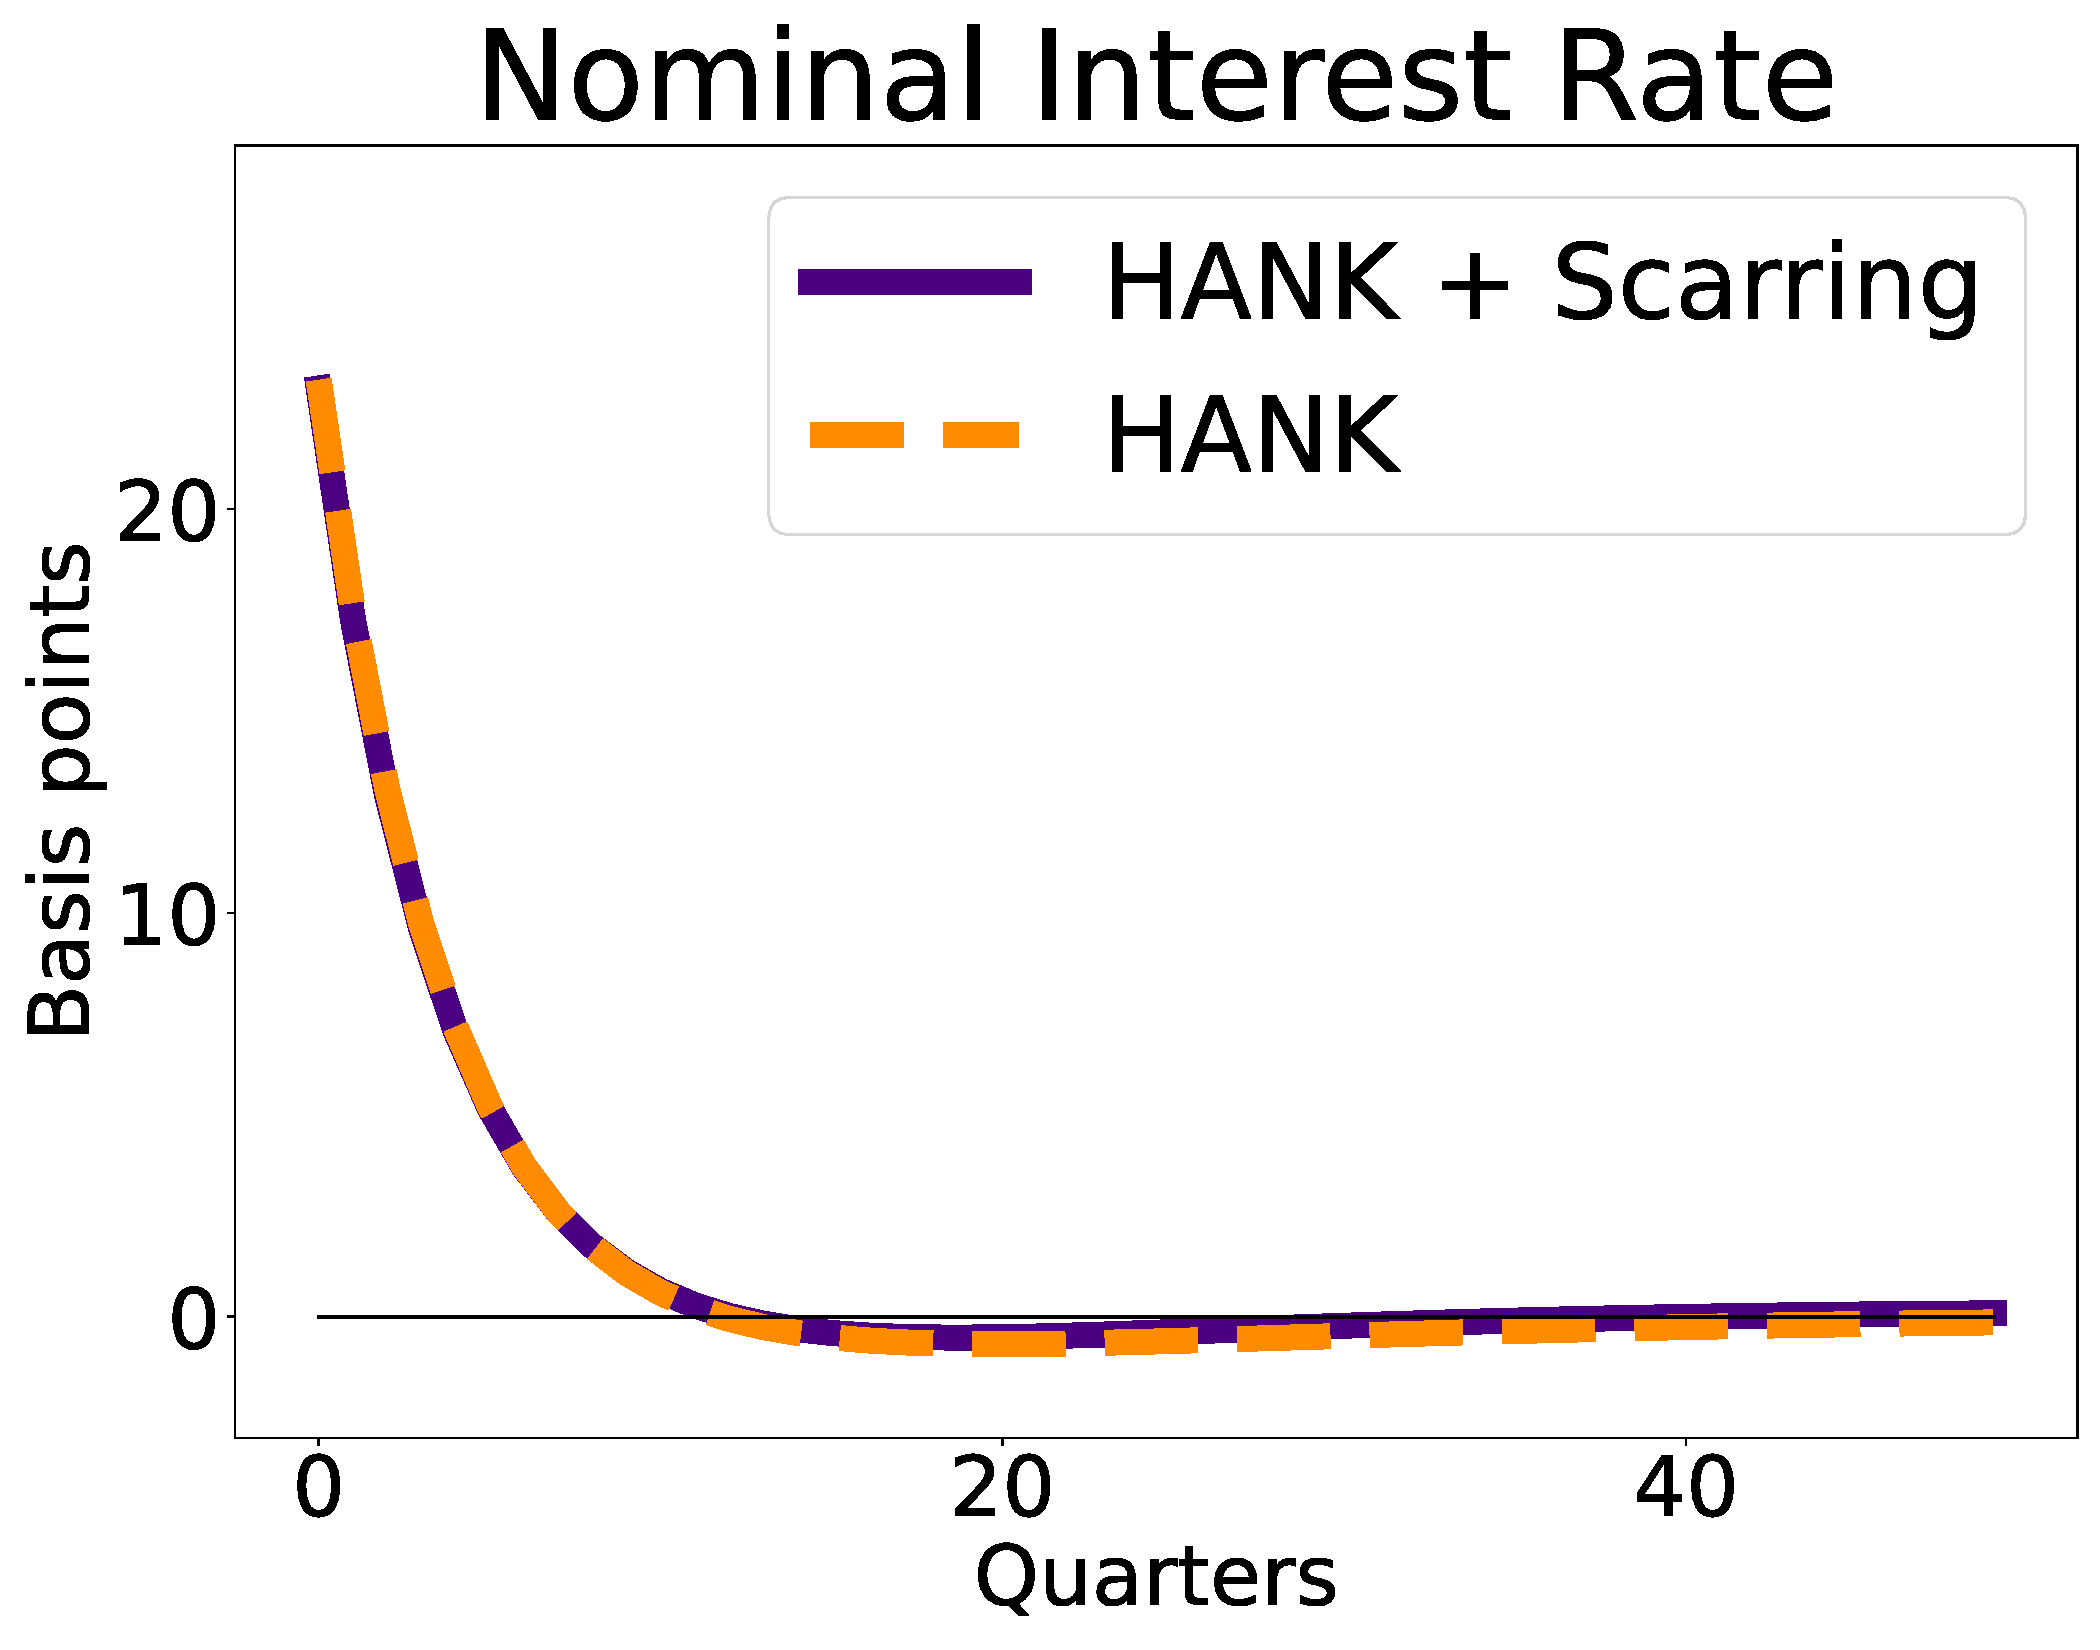
\includegraphics[scale=.14]{text/Chapter1/Figures/IPRs_ev/i_IPR_ev}
  \label{fig:1}
\end{minipage}\hfil % <-- added
\begin{minipage}{0.33\textwidth}
  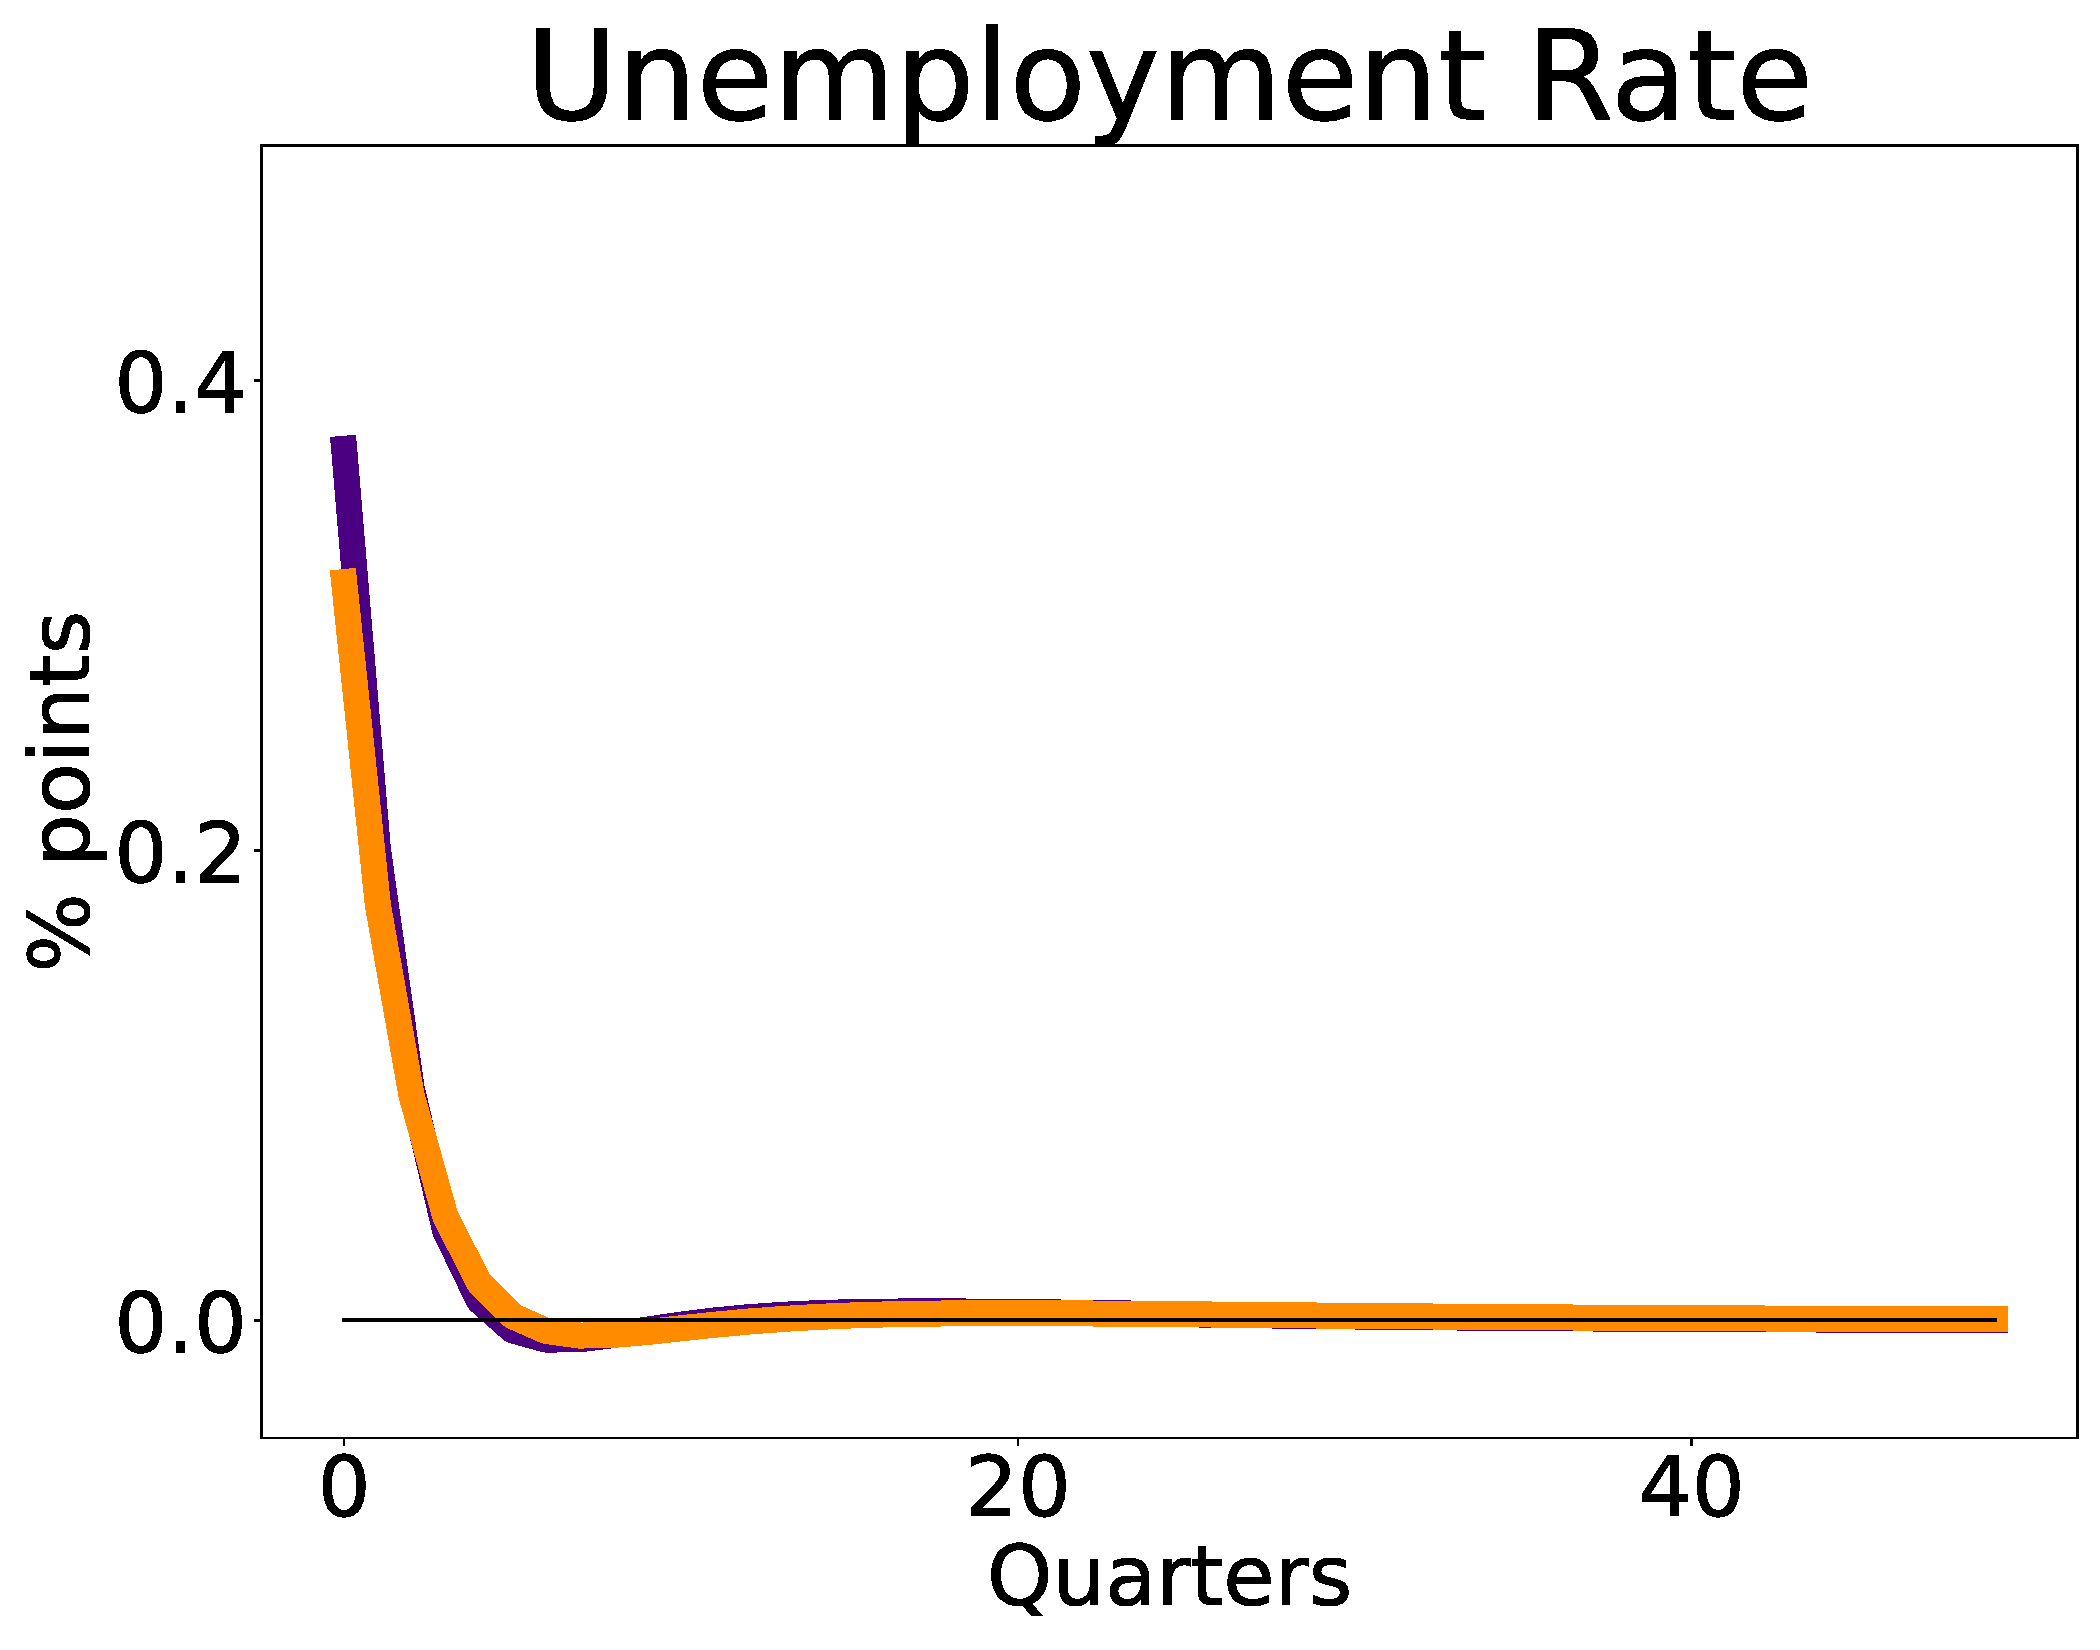
\includegraphics[scale=.14]{text/Chapter1/Figures/IPRs_ev/U_IPR_ev}
  \label{fig:2}
\end{minipage}\hfil % <-- added
\begin{minipage}{0.33\textwidth}
  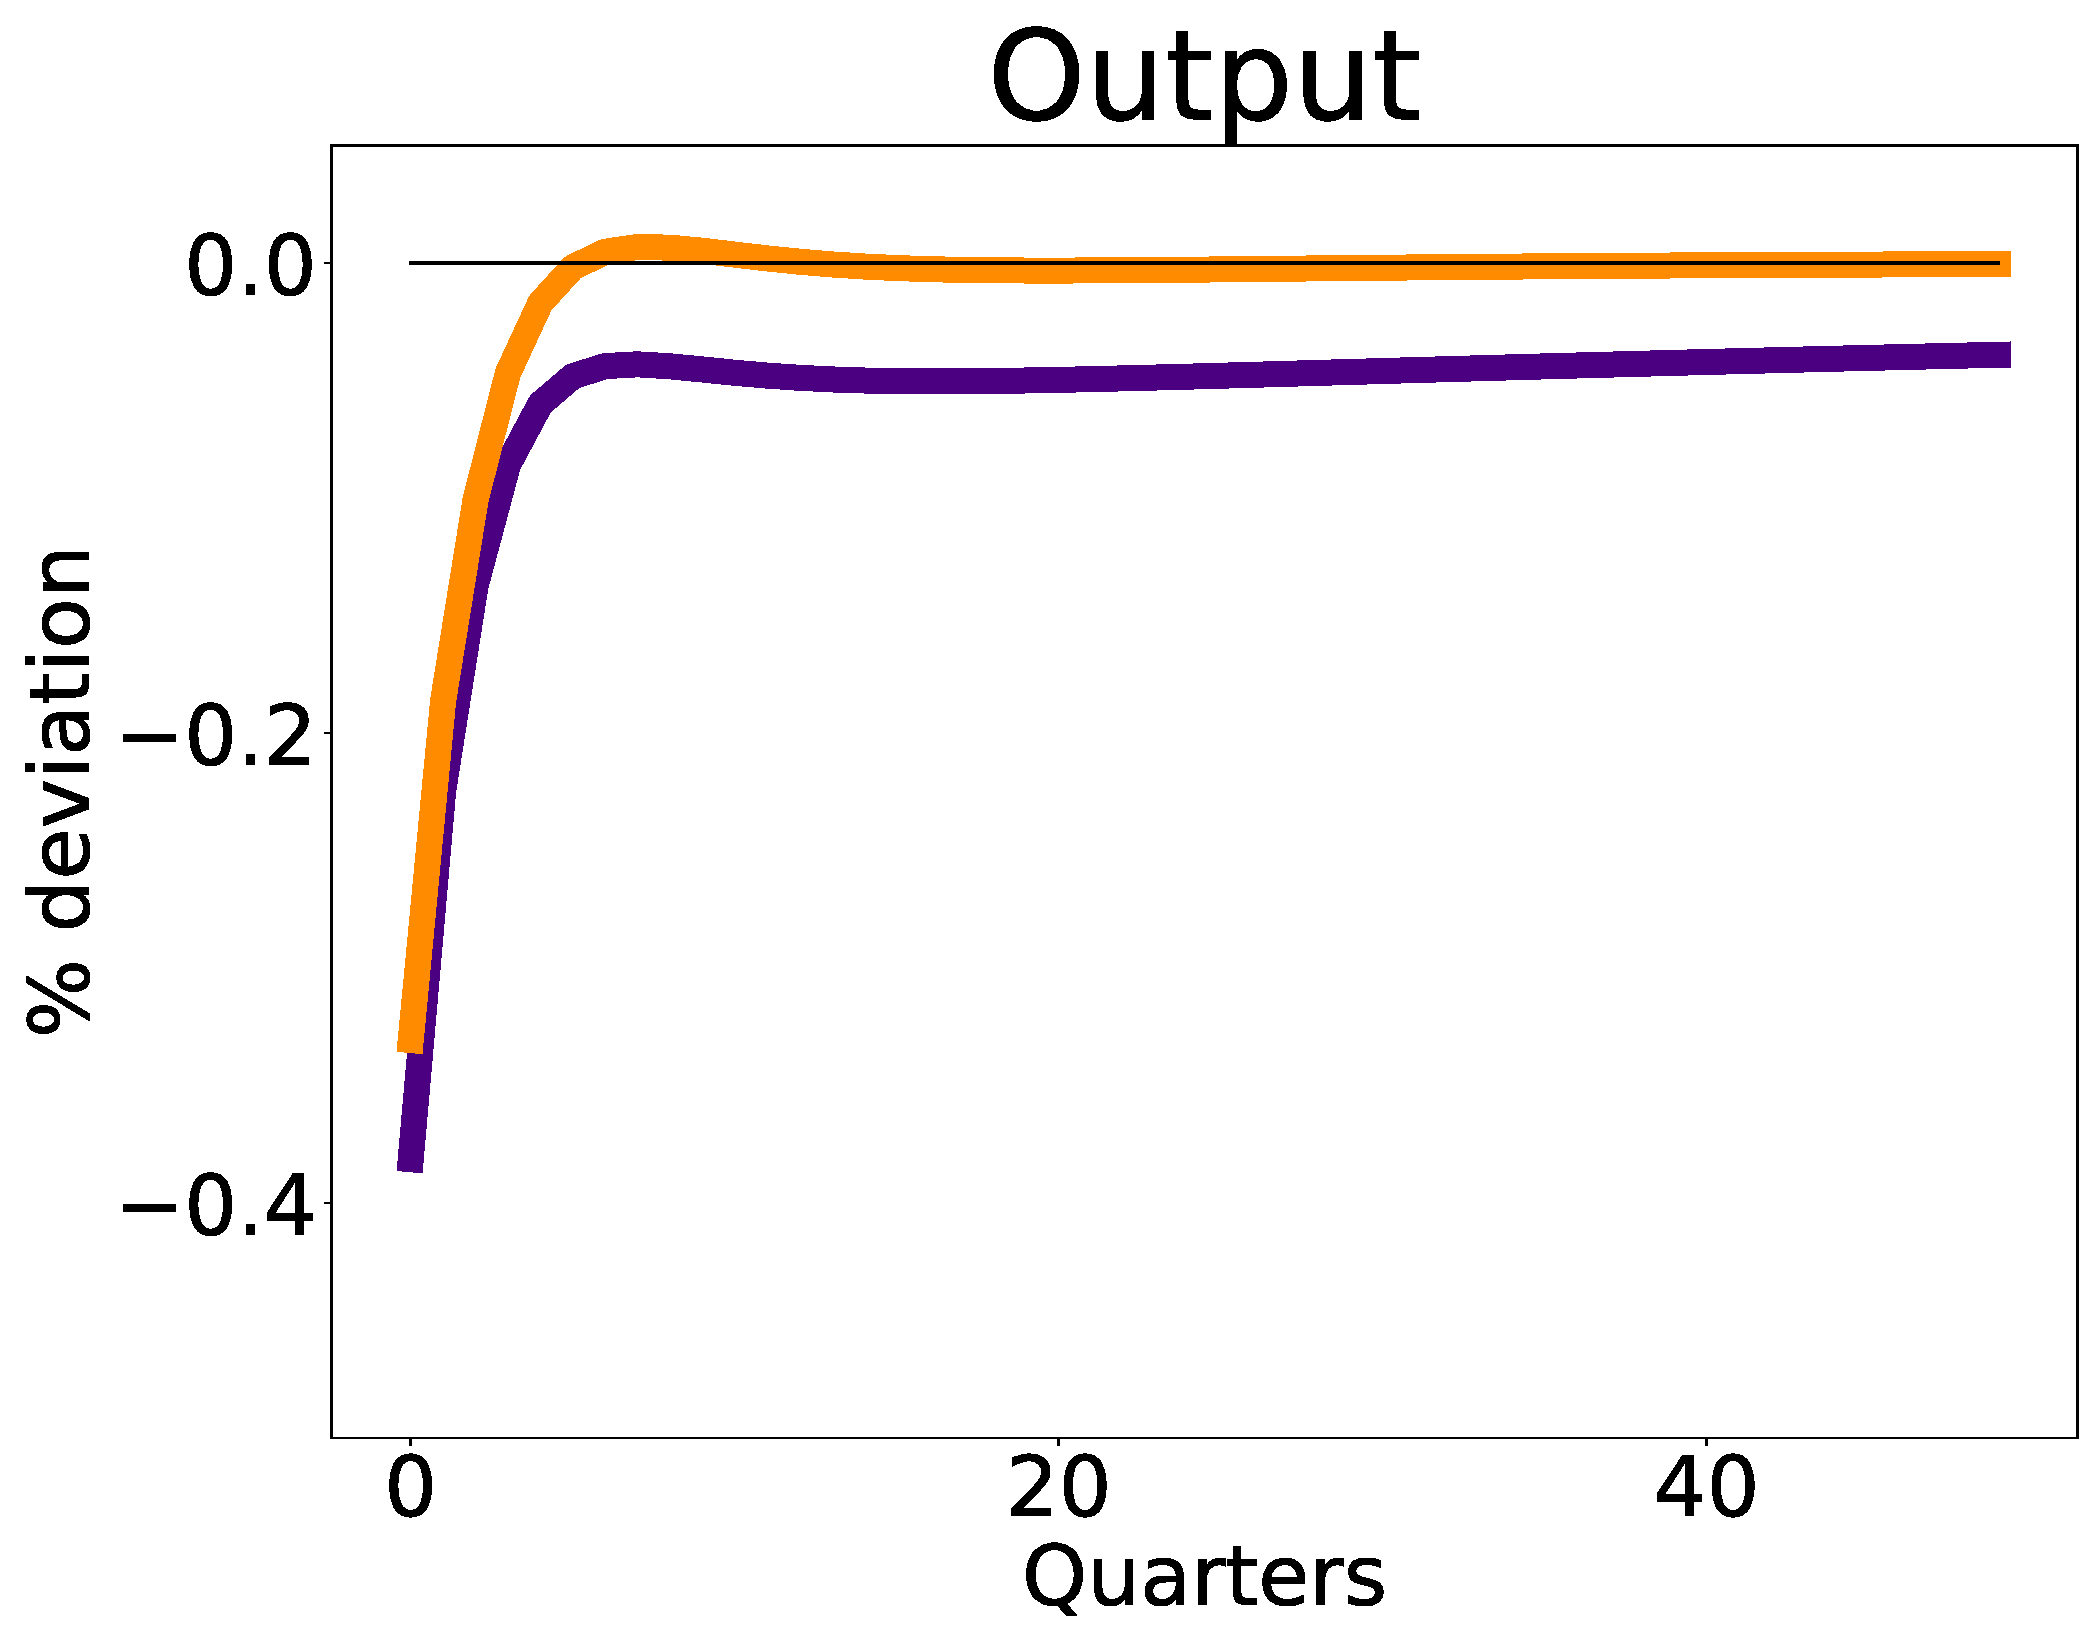
\includegraphics[scale=.14]{text/Chapter1/Figures/IPRs_ev/Y_IPR_ev}
  \label{fig:3}
\end{minipage}
\begin{minipage}{0.33\textwidth}
  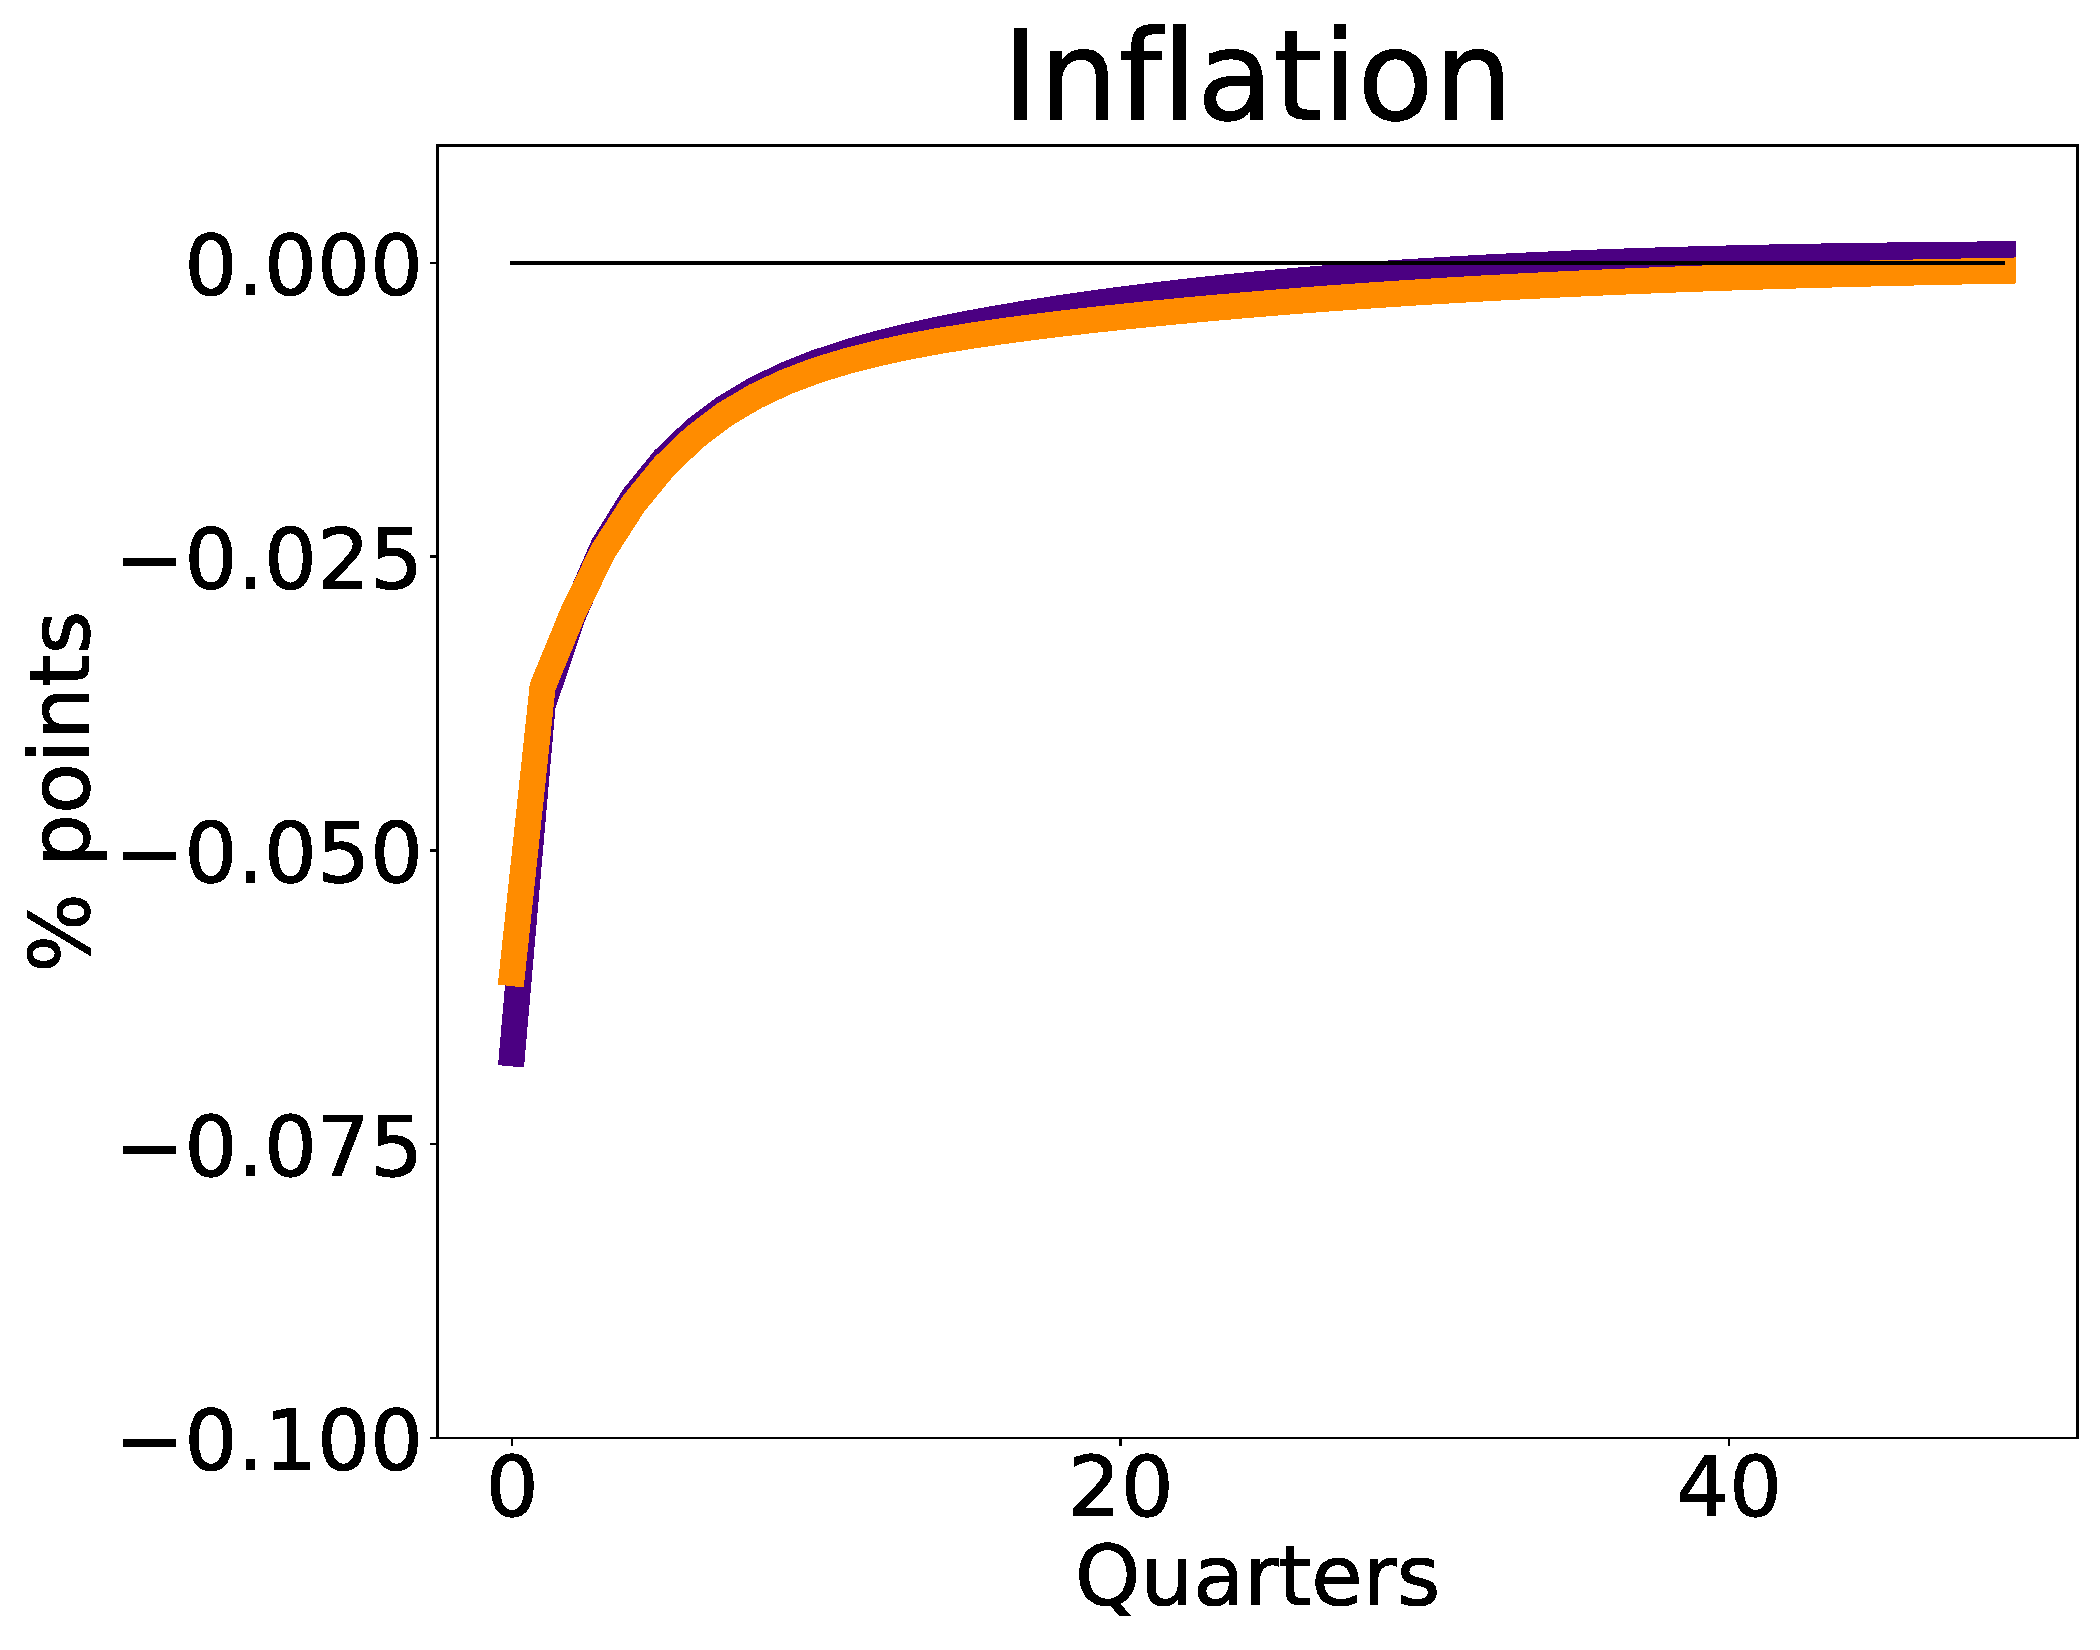
\includegraphics[scale=.14]{text/Chapter1/Figures/IPRs_ev/pi_IPR_ev}
  \label{fig:4}
\end{minipage}
\medskip
\begin{minipage}{0.33\textwidth}
  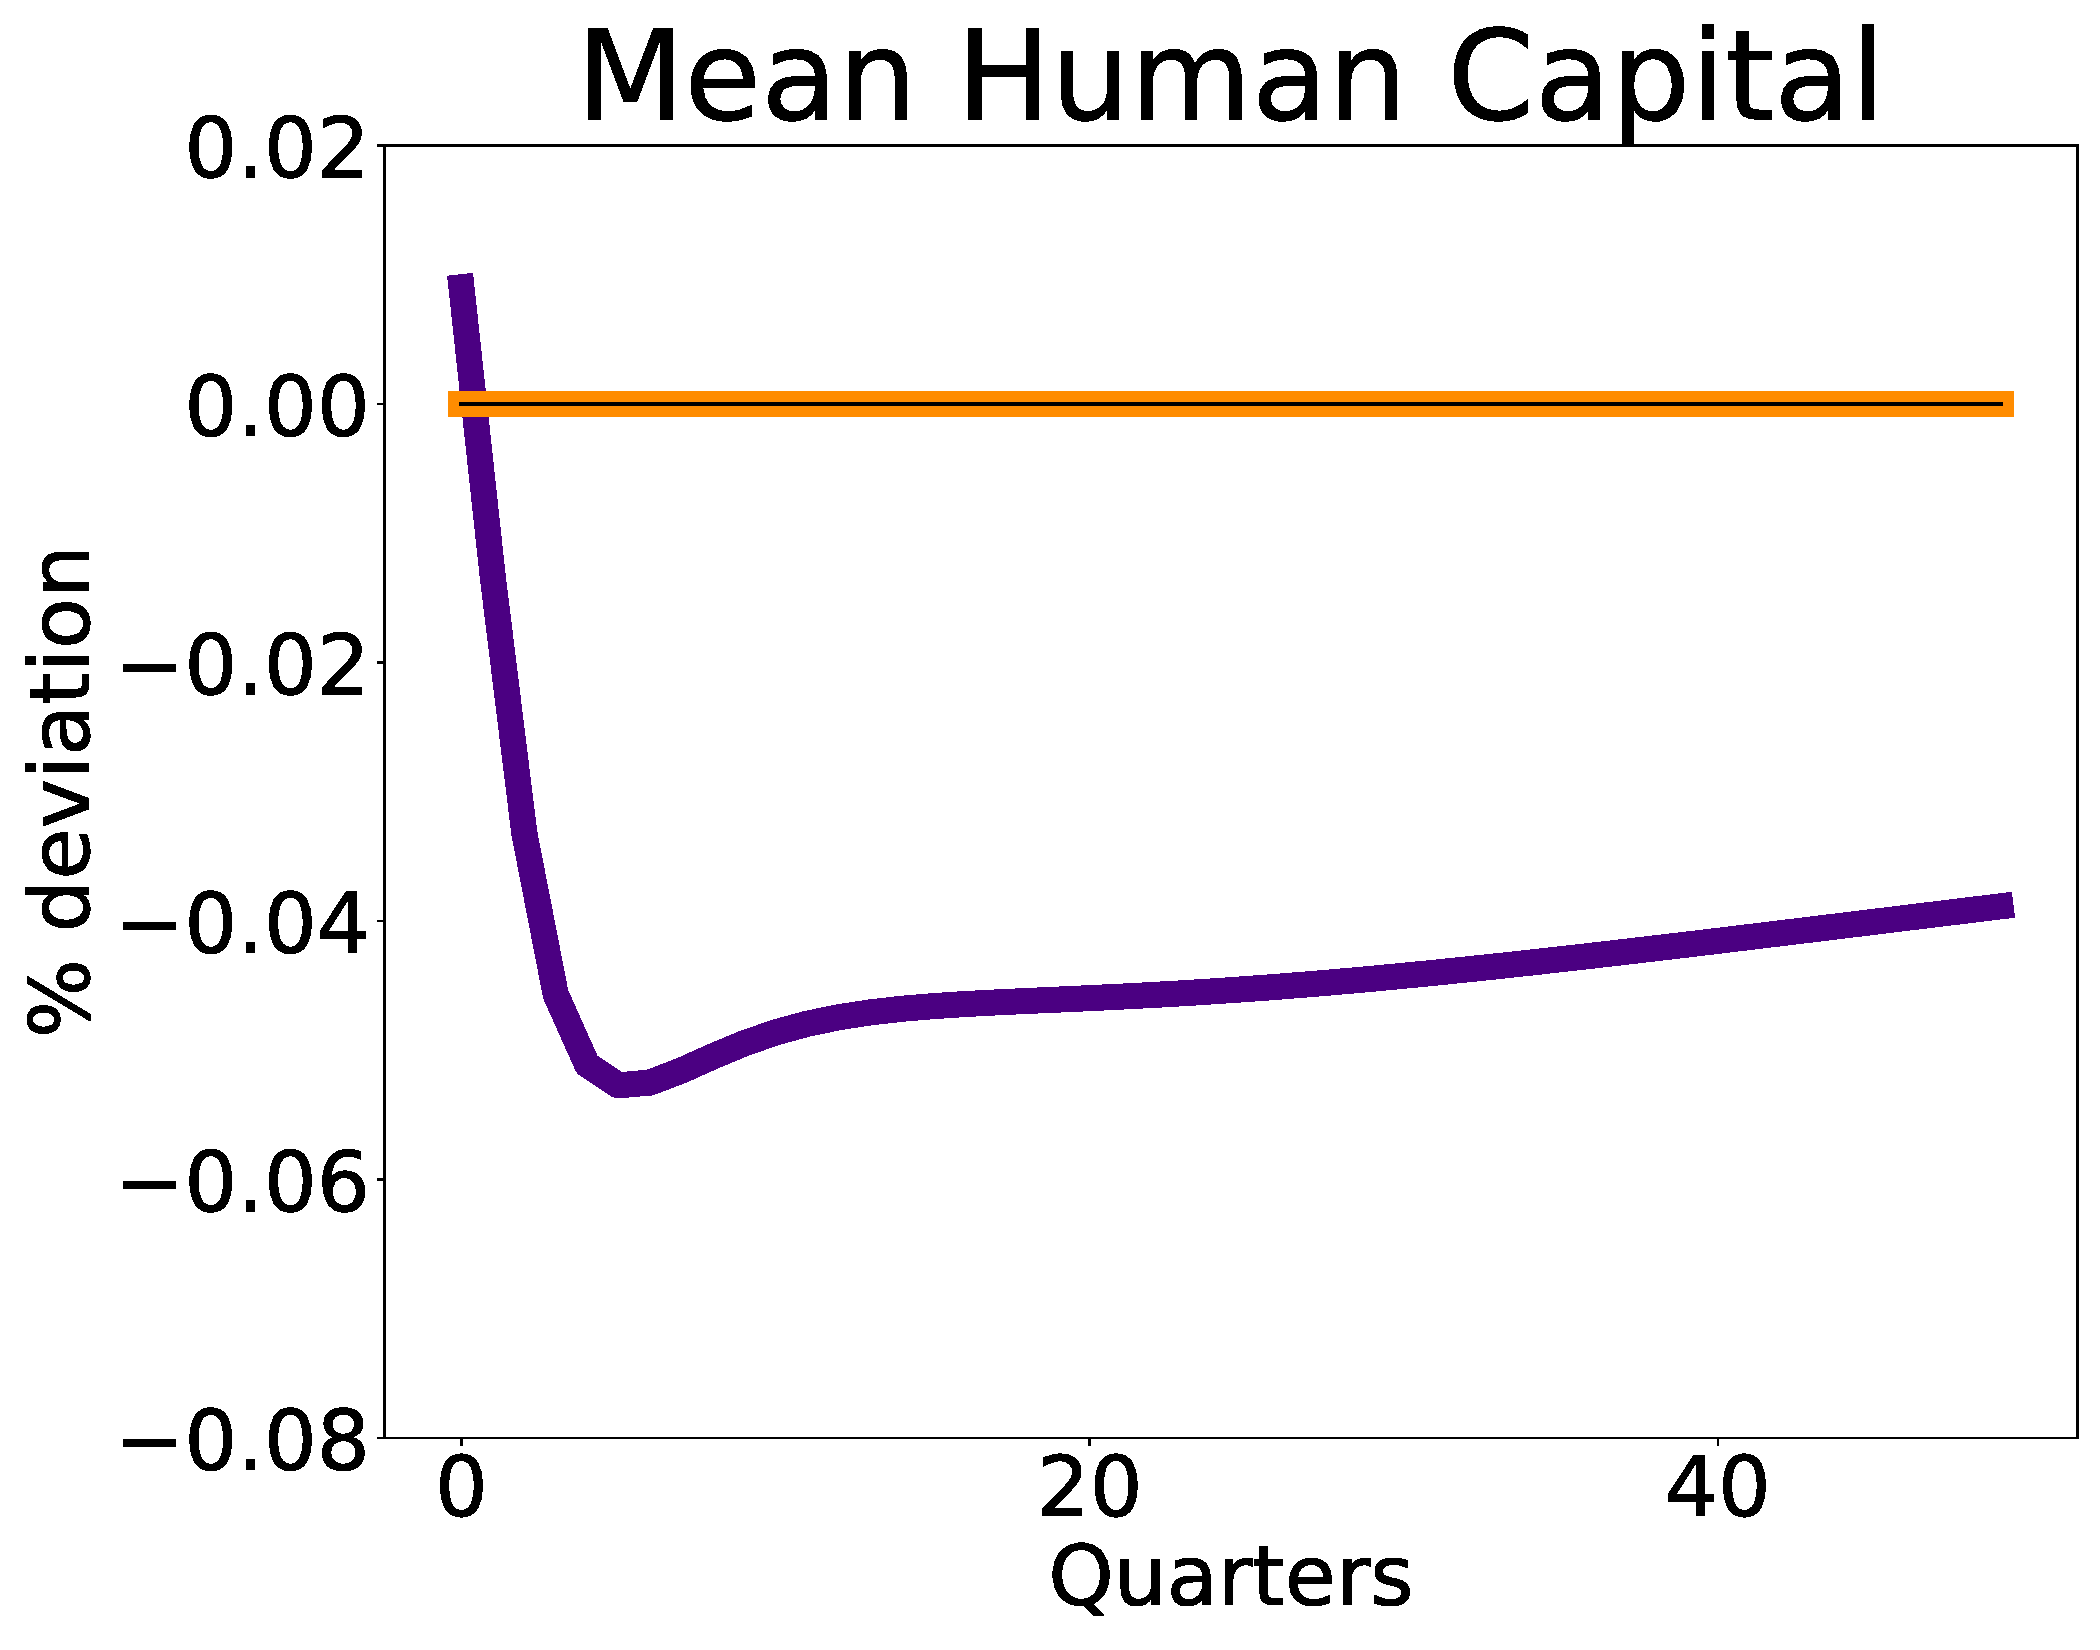
\includegraphics[scale=.14]{text/Chapter1/Figures/IPRs_ev/H_E_IPR_ev}
  \label{fig:4}
\end{minipage}\hfil % <-- added
\begin{minipage}{0.33\textwidth}
  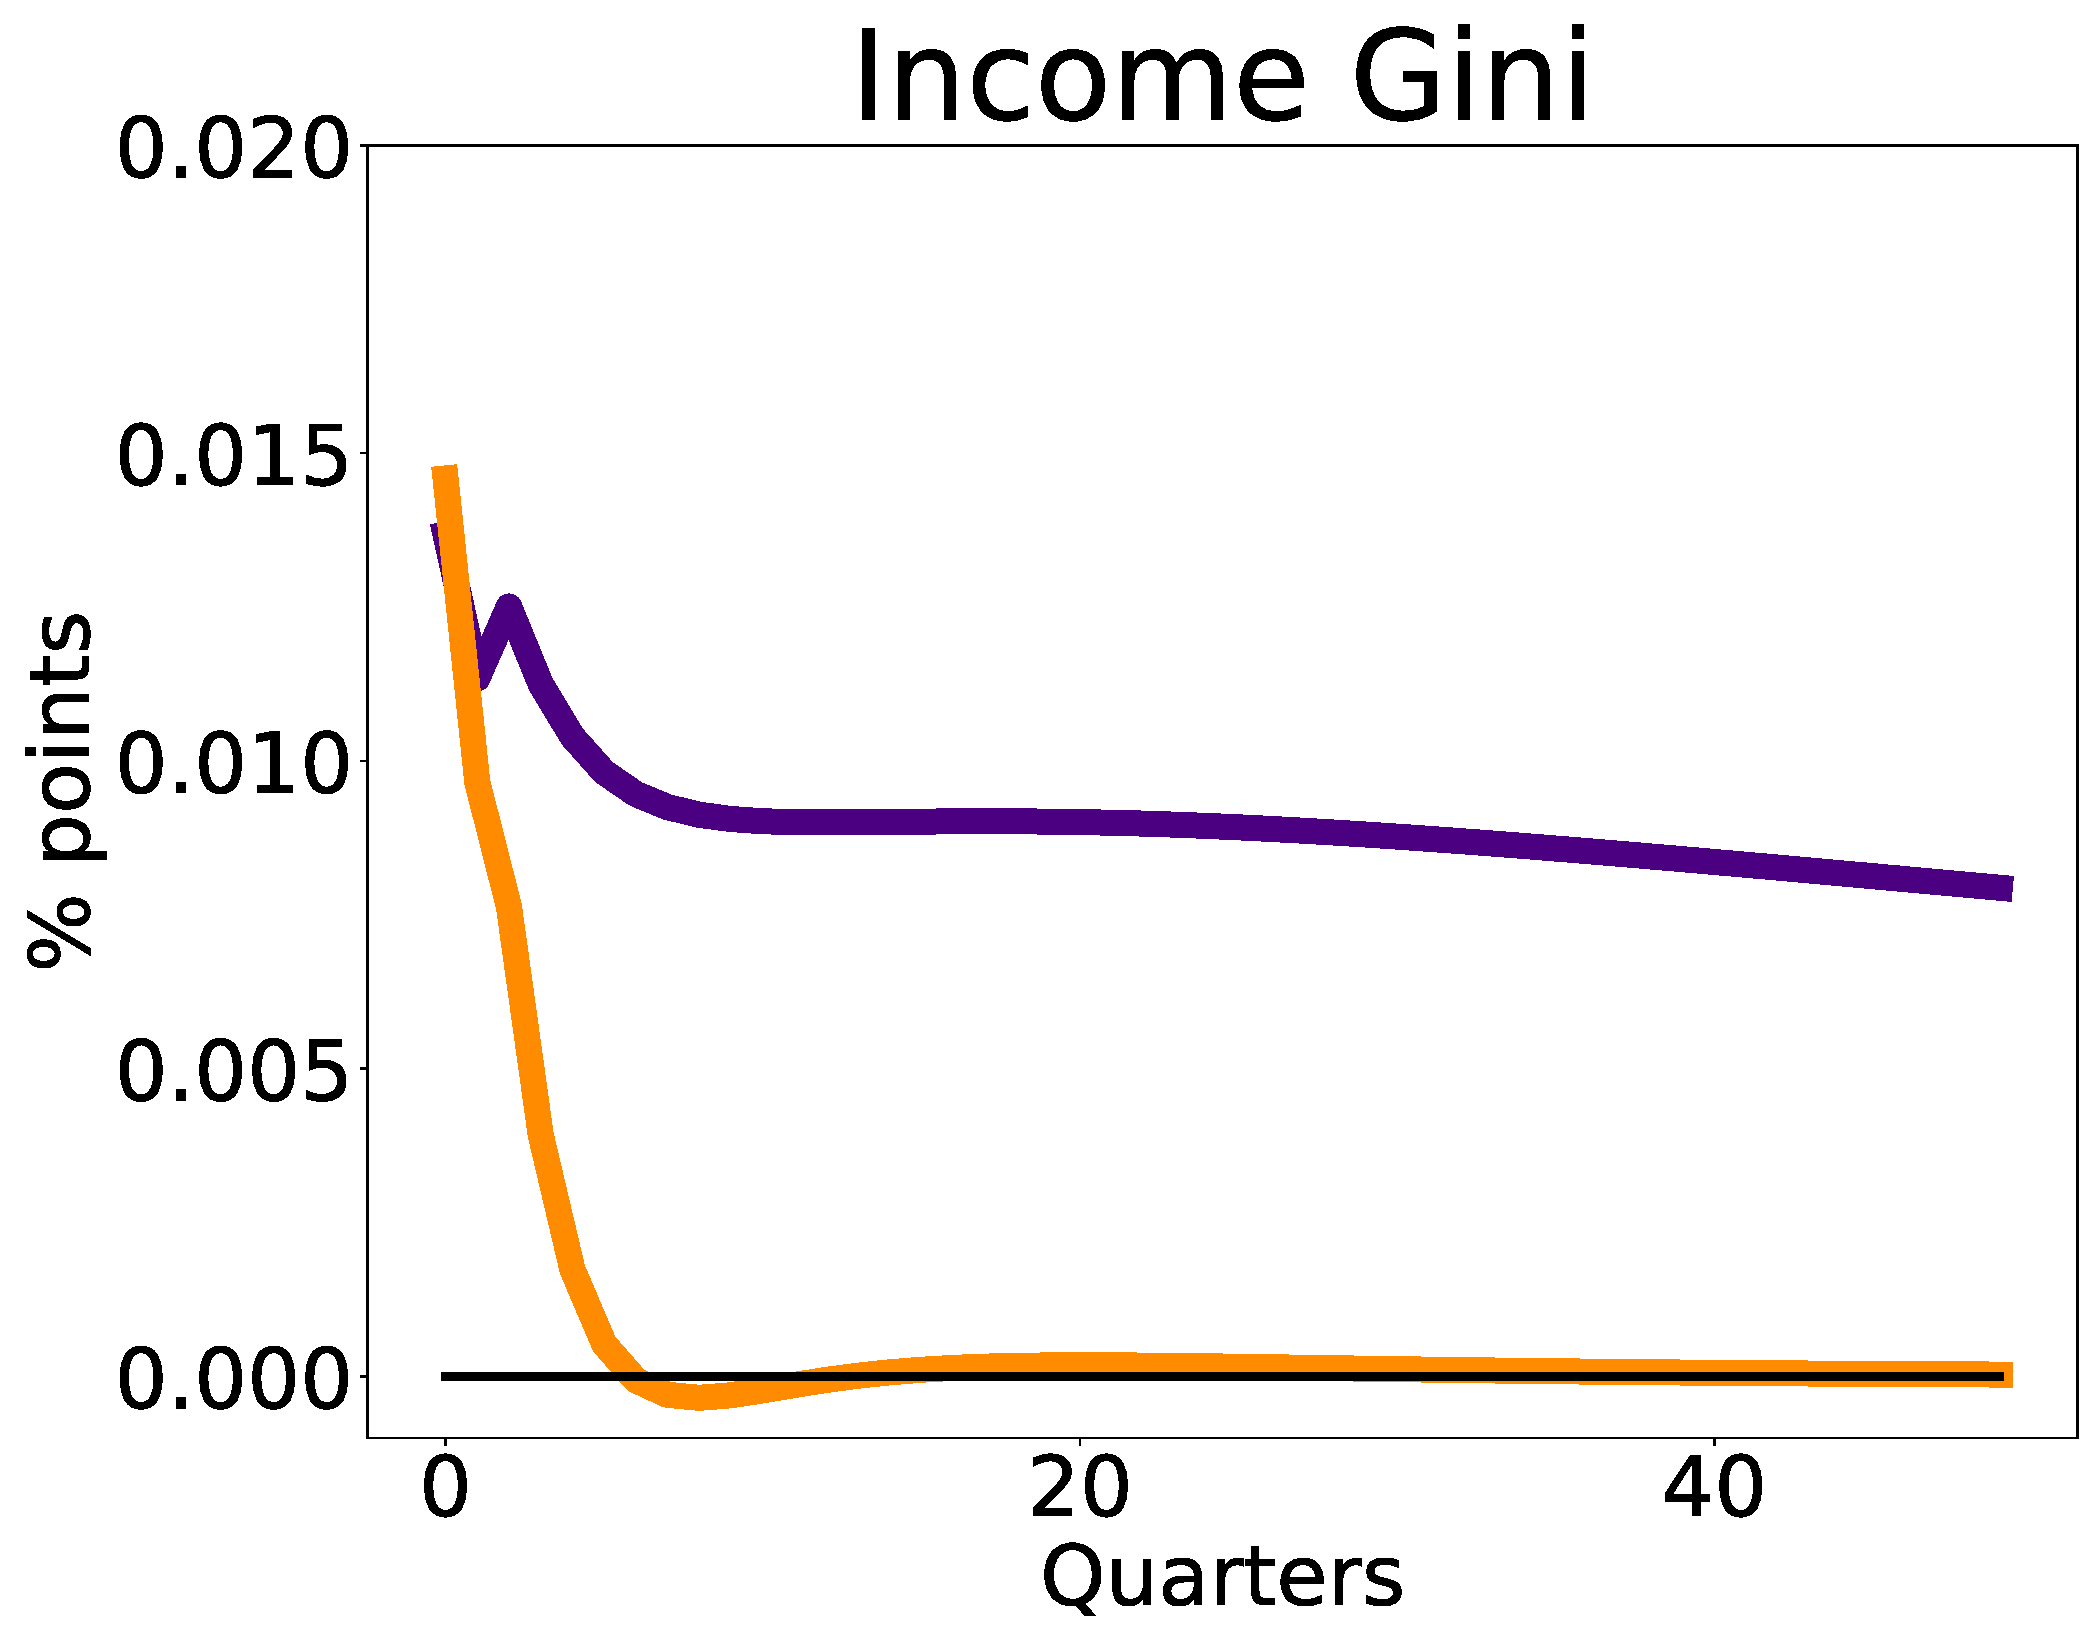
\includegraphics[scale=.14]{text/Chapter1/Figures/IPRs_ev/gini_IPR_ev}
  \label{fig:5}
\end{minipage}\hfil % <-- added
\caption{Impulse responses to a monetary policy shock} 
\floatfoot{Note: The exercise above plots the impulse responses to a 25 basis point shock to the Taylor rule. I assume that the Taylor rule now is $i_{t} =r^{*} +  \phi_{ev} i_{t-1} + (1-\phi_{ev})(\phi_{\pi} \pi_{t}  + \phi_{Y} (Y_{t} -  Y_{ss})) + \epsilon^{m}_{t}$ where I set  $\phi_{ev} = 0.8$ as in \cite{Bardoczy2020}}
\label{IPR_ev}
\end{figure}


\subsection{Self Defeating Fiscal Consolidation}

The idea of self defeating fiscal consolidation in the presence of hysteresis was proposed by \cite{FATAS2018} in a simple toy model. This section shows that fiscal consolidation is indeed substantially less effective at reducing the debt-to-GDP ratio when hysteresis is calibrated to microeconomic evidence on unemployment scarring. I consider a decrease in government spending shock that is $1\%$ of GDP with a quarterly persistence of the shock is 0.933. Figure \ref{Fiscal_Consolidation} plots responses of relevant variables to this shock. With unemployment scarring, debt to GDP falls substantially less in response to a decrease in government spending and in the long run increases. The initial jump in debt to GDP is due to the model featuring realistic aggregate MPCs. In the long run, debt to GDP rises because of persistent losses in tax revenues. For debt to GDP, scarring drives both persistent losses in output as well as the increased pressure on debt to rise. The bottom right panel plots the response of the Gini index to the negative government spending shock and shows that fiscal consolidation almost permanently raises income inequality. In particular, a one percentage point decrease in government spending increases the income Gini index by 0.05 percentage points.



\begin{figure}[!t]
\begin{center}
\begin{minipage}{0.5\textwidth}
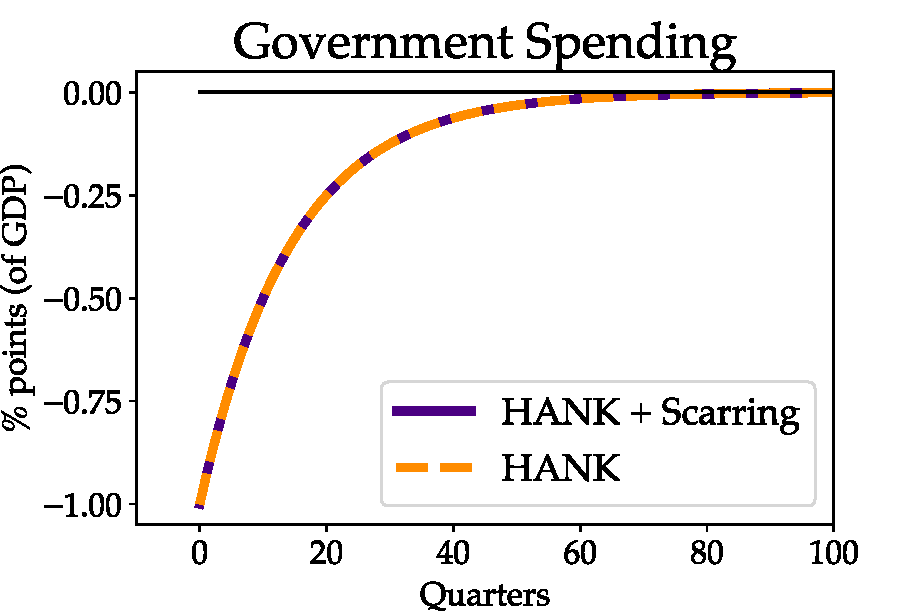
\includegraphics[scale=.5]{text/Chapter1/Figures/Fiscal_Consolidation/Government_spending_FC}
\end{minipage}\hspace*{\fill}
\begin{minipage}{0.5\textwidth}
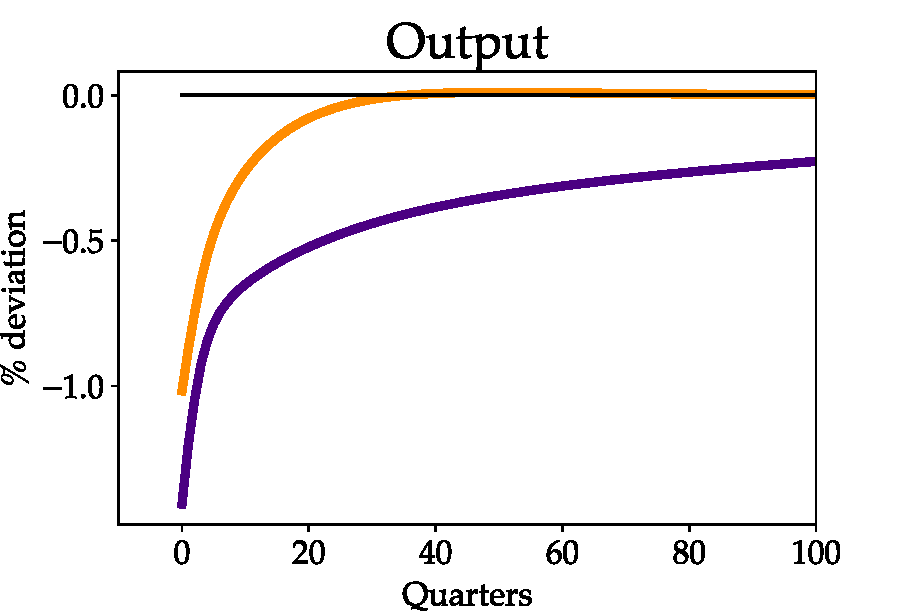
\includegraphics[scale=.5]{text/Chapter1/Figures/Fiscal_Consolidation/Output_FC}
\end{minipage}
\medskip
\begin{minipage}{0.5\textwidth}
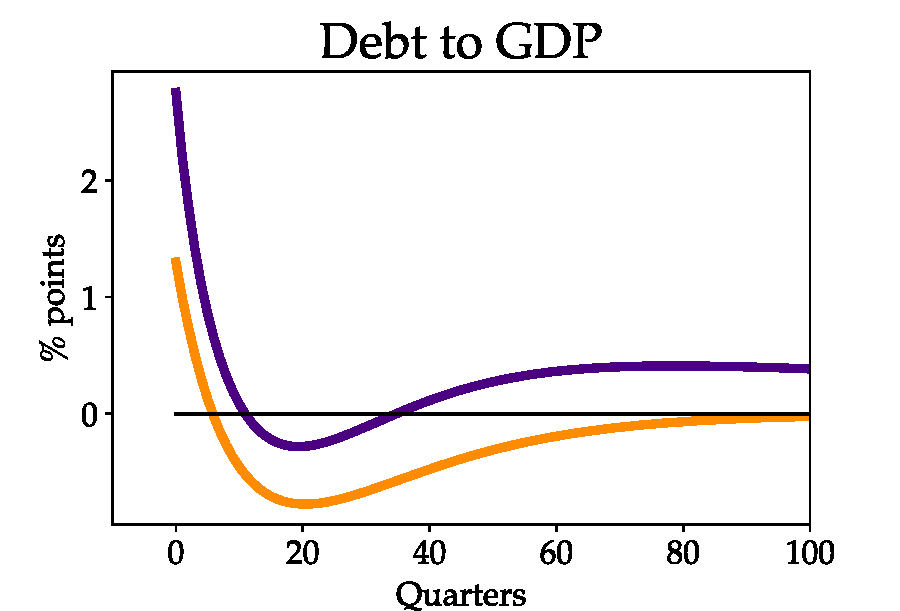
\includegraphics[scale=.5]{text/Chapter1/Figures/Fiscal_Consolidation/debt to GDP_FC}
\end{minipage}\hspace*{\fill}
\begin{minipage}{0.5\textwidth}
\includegraphics[scale=.5]{text/Chapter1/Figures/Fiscal_Consolidation/gini_FC}
\end{minipage}
\caption{Responses to a negative government spending shock} 
\floatfoot{Note: This exercise plots the impulse responses to a one percentage point decrease in government spending $G_{t}$ with AR(1) persistence 0.9.}

\label{Fiscal_Consolidation}
\end{center}
\end{figure}



\subsection{Overview of the Model}

\begin{figure}[H]
    \begin{tikzpicture}[>=stealth', shorten >=1pt, auto,
    node distance=2.5cm, 
    transform shape, align=center, 
    state/.style={circle, draw,  minimum size=2cm}, every node/.style={scale=1.5}]
    \node[state]    (C) {households};  
    \node[state, left=of C] (i) {Demand \\ Shock};
    \node[state,  right=of C] (Y) {Producers};
    \node[state, below = of C ] (JF) {Matching};
    \node[state, left = of JF ] (G) {Gov.\\Budget};
    \path[->] (i) edge node {} (C)
              (C) edge node {} (Y)
              (Y) edge node {} (JF)
              (JF) edge node {} (C)
              (JF) edge node {} (G)
              (G) edge node {} (C)
              (C) edge node {} (G);
  \draw  (i) -- node [above] {$\uparrow \beta$} (C);
  \draw  (C) -- node [above] {$\downarrow C$} (Y);
  \draw  (JF) -- node [left] {$\uparrow U$} (C);
  \draw  (Y) -- node [right] {$\downarrow v$} (JF);
  \draw  (JF) -- node [above] {$\uparrow U$} (G);
  \draw  (G) -- node [left] {$\uparrow \tau$ $\uparrow A$ $\uparrow B$ }(C);
  \draw  (C) -- node [below] {} (G);
  \draw[->,red] (JF) to[bend right] node[right] {$\downarrow h$} (C);
  \draw[->,red] (JF) to[bend left] node[below] {$\downarrow h$} (G);
  \draw[->,red] (JF) to[bend right] node[right] {$\downarrow h$} (Y);
\end{tikzpicture}
\end{figure}



